% =====================================================================
%  Sections 3 (Method) and 4 (Experiments), English — ICAIF 8-page budget
%
%  Include with: % =====================================================================
%  Sections 3 (Method) and 4 (Experiments), English — ICAIF 8-page budget
%
%  Include with: % =====================================================================
%  Sections 3 (Method) and 4 (Experiments), English — ICAIF 8-page budget
%
%  Include with: % =====================================================================
%  Sections 3 (Method) and 4 (Experiments), English — ICAIF 8-page budget
%
%  Include with: \input{sections/03-04-en}
%  Packages: booktabs, graphicx, amsmath, array
%  Figures:  figures/  (three figures only)
%
%  Length target: Section 3 ~1.6 pp + Section 4 ~2.4 pp = ~4 pp,
%  leaving 3 pp for Sections 1-2 and 1 pp for Section 5 and references.
% =====================================================================

\section{Method: SPR-IRL}
\label{sec:method}

This section defines Symmetric Preference Recovery (SPR-IRL). SPR-IRL is not a
single model but a procedure comprising (i) symmetric estimation over shared
features, (ii) out-of-sample stability assessment, and (iii) a contrast against
sign expectations fixed in advance.

\subsection{Continuous Action and Symmetric Estimation}
\label{sec:setup}

Let the investor types be
$\mathcal{I}=\{\text{foreign},\text{institutional},\text{retail}\}$. Writing
$V^{buy}_{i,t}$ and $V^{sell}_{i,t}$ for the daily gross buy and sell value of
type $i$, the action is
\begin{equation}
u_{i,t}=\frac{V^{buy}_{i,t}-V^{sell}_{i,t}}
             {V^{buy}_{i,t}+V^{sell}_{i,t}}\in[-1,1].
\label{eq:action}
\end{equation}
Because the denominator is the type's own gross turnover rather than
market-wide turnover, $u_{i,t}$ is a common scale unaffected by differences in
trading size across types, and unlike a binary label it preserves intensity.

All three types receive the same state features $x_{i,t}\in\mathbb{R}^{3}$, the
same context $C_t\in\mathbb{R}^{2}$, and the same model form; only the
parameters $\theta_i=(\beta_i,B_i,\alpha_i)$ are estimated separately on each
type's own data. Since no type is assigned a different feature a priori, any
difference in the results is learned rather than imposed, and this is what
licenses direct comparison of coefficients across types.

The training sample is $(x_{i,t},C_t,a_{i,t+1})$ with $a_{i,t+1}=u_{i,t+1}$: a
day-$t$ state explains day-$t+1$ behaviour, so no future trade enters the
features.

\subsection{Reward Features and Market Context}
\label{sec:features}

All three features and both contexts are standardized on the training indices of
each split only, so every coefficient reads as the effect of a
one-standard-deviation move.

\textbf{(F1) Medium-term momentum} $x^{mom}_{t}=\log(P_t/P_{t-20})$. The 20-day
window is pre-specified for interpretability and was not tuned on the data. A
positive coefficient indicates trend following and a negative one contrarian
trading; the sign expectation follows the literature on type-specific momentum
trading~\cite{grinblatt2000investment,choe1999foreign}.

\textbf{(F2) Herding} is the cross-sectional average of the previous day's
actions of the two types other than $i$,
\begin{equation}
x^{herd}_{i,t}=\tfrac{1}{2}\left(u_{j,t-1}+u_{k,t-1}\right),\qquad j,k\neq i.
\label{eq:herd}
\end{equation}
The one-day lag is not an information constraint but a design choice that keeps
the same-day accounting offset between types out of the predictor set
(\S\ref{sec:beta}). The sign expectation follows the institutional herding
literature~\cite{lakonishok1992impact}, which however measures herding
\emph{within} the institutional group whereas Equation~\eqref{eq:herd} measures
a relation \emph{between} types.

\textbf{(F3) Underwater gap} uses an average-cost proxy $\bar P_{i,t}$ and the
day's gross-trade VWAP $P^{vwap}_{i,t}$,
\begin{equation}
x^{uw}_{i,t}=\max\!\left(
\frac{\bar P_{i,t}-P^{vwap}_{i,t}}{\bar P_{i,t}},\,0\right).
\label{eq:underwater}
\end{equation}
Truncation at zero makes the variable reference-point dependent by construction.
The average cost recursively updates an effective inventory from gross
quantities and values, multiplying the previous day's inventory by a forgetting
factor $\rho=0.98$ (half-life about 34 trading days). The sign expectation
follows the disposition-effect
literature~\cite{shefrin1985disposition,odean1998investors}. Because the proxy is
built from aggregate flow, the coefficient on $x^{uw}$ cannot be read as a direct
test of that effect.

\textbf{The context} consists of the one-day KOSPI200 return $r_t$ and the
KRW/USD level $z_t=(\log e_t-\mu_{t-1,252})/\sigma_{t-1,252}$, where the mean and
standard deviation use only data through $t-1$. Because Samsung Electronics
carries a large KOSPI200 weight, stock momentum overlaps the market return and
feature--context correlations range from $-0.29$ to $0.22$; individual
coefficients are therefore conditional associations given the other terms.

\subsection{Myopic Reward and the Reduction to Lasso}
\label{sec:model}

Define the action score of type $i$ as
\begin{equation}
q_{i,t}=(\beta_i+B_iC_t)^{\top}x_{i,t}+\alpha_i^{\top}C_t.
\label{eq:score}
\end{equation}
Here $\alpha$ is a level effect that shifts behaviour even at average features
and $B$ a slope effect that changes feature sensitivity across contexts.
Including interactions while omitting the lower-order term $C_t$ is a standard
specification error, so the inclusion of $\alpha$ is not something to justify
empirically. With the one-step reward
$R_i=q_{i,t}a-\tfrac{\kappa}{2}a^{2}$ the optimal policy is
\begin{equation}
a^{*}_{i,t+1}=\mathrm{clip}(q_{i,t}/\kappa,-1,1).
\label{eq:policy}
\end{equation}
Without the quadratic term the solution would be $\pm1$ almost always and
intensity could not be reproduced. We fix $\kappa=1$ for identification, which
normalizes the units of the reward and the coefficients rather than asserting
that the empirical curvature is one. The training objective is
\begin{equation}
\min_{\theta_i}\ \frac{1}{|\mathcal{D}_i|}
\sum_{t\in\mathcal{D}_i}\!\bigl(a^{*}_{i,t+1}-a_{i,t+1}\bigr)^{2}
+\lambda_i\lVert\theta_i\rVert_1,
\label{eq:loss}
\end{equation}
optimized independently per type with Adam~\cite{kingma2015adam}.

\begin{proposition}[Reduction to Lasso]
\label{prop:lasso}
Let
$z_{i,t}=[\,x_{i,t};\ \mathrm{vec}(x_{i,t}C_t^{\top});\ C_t\,]\in\mathbb{R}^{11}$
and $\theta_i=[\,\beta_i;\ \mathrm{vec}(B_i);\ \alpha_i\,]$, so that
$q_{i,t}=\theta_i^{\top}z_{i,t}$. If $|q_{i,t}|\le 1$ throughout the training
sample, the clip in Equation~\eqref{eq:policy} never binds, $a^{*}=q$, and
Equation~\eqref{eq:loss} becomes exactly an $L_1$-penalized (Lasso) regression of
$a_{i,t+1}$ on $z_{i,t}$.
\end{proposition}

In our sample the maximum $|q|$ is 0.842 for foreign, 0.587 for retail and 0.135
for institutional investors, and the saturation rate is exactly zero in all 45
splits, so the premise holds. In SPR-IRL, ``recovering a preference'' and
``regressing order flow'' are therefore numerically indistinguishable.

This is not a defect but a consequence of myopia. If the agent looks one step
ahead, today's action does not affect anything beyond tomorrow, so what the agent
wants (the reward) collapses onto what it does (the policy). Applying the
stochastic policy of maximum-entropy IRL~\cite{ziebart2008maximum},
$\pi\propto\exp(R/\tau)$, makes $\pi$ a truncated normal with mean $q$ whose
point estimate coincides with the above; the reduction is thus a property of the
myopic, quadratic-reward setting in general. The value of the IRL formulation
lies in the extension path: once state dynamics and multi-period value are
introduced, the reward separates from the policy and yields a structural recovery
that regression cannot reach (\S\ref{sec:discussion}).

\subsection{Validation Protocol}
\label{sec:protocol}

Rather than reporting the recovered coefficients as they are, we apply four
stages. \textbf{(V1)} Combinatorial purged
cross-validation~\cite{lopez2018advances} with ten temporal folds of which two
are test folds gives $\binom{10}{2}=45$ splits, with a one-day purge, a five-day
embargo, and all standardization fitted on training indices only. Because splits
share observations, sign consistency is interpreted as a stability indicator, not
a $p$-value. \textbf{(V2)} To address that limitation we partition the sample
into calendar-month blocks, resample 1{,}000 times, and obtain 95\% confidence
intervals; month blocks preserve the autocorrelation of daily flow within each
block. \textbf{(V3)} Because CPCV can place a test fold before a training fold,
we add an expanding walk-forward: train on the first 400 observations, predict
the next 60 trading days after a five-day purge, and repeat while expanding by 60
days, for ten windows. \textbf{(V4)} To confirm the results are not an artefact
of the $L_1$ penalty we re-estimate under $L_2$ and no penalty and compare signs.

Metrics are MAE, RMSE, directional accuracy (the fraction with
$\mathrm{sign}(a^{*})=\mathrm{sign}(a)$), the actual--predicted correlation, and
the saturation rate. Because action standard deviations differ across types,
absolute errors are not compared across types. As a naive reference we report a
persistence rule that predicts the previous day's own action.

% =====================================================================
\section{Experiments}
\label{sec:experiments}

\subsection{Data}
\label{sec:data}

From daily records for Samsung Electronics (005930) we use the most recent 973
rows for which the 252-day exchange-rate history, the 20-day momentum, and the
next day's action can all be computed; state dates run 2022-01-06 to 2025-12-29.
The single-stock design is not a sample limitation but a controlled setting that
removes stock fixed effects and liquidity differences and isolates preference
heterogeneity across types.

Mean actions are near zero for all three types, but standard deviations differ
(retail 0.334, foreign 0.257, institutional 0.125) and first-order
autocorrelations are 0.345, 0.401 and 0.149. Same-day actions across types are
strongly negatively related (foreign--retail $-0.772$, institutional--retail
$-0.499$), reflecting the market-clearing constraint that one type's buying must
appear as another's selling; this bounds the interpretation in \S\ref{sec:beta}.

Training settings are, per type, foreign 75 epochs / batch 256 / lr 0.001 /
$\lambda=0$; institutional 10 / 2048 / 0.0005 / 0.01; retail 20 / 512 / 0.001 /
0.0003, with seed 42, $\kappa=1$, and 11 parameters per type ($\beta$ 3, $B$ 6,
$\alpha$ 2).

\subsection{Out-of-Sample Behaviour Reproduction}
\label{sec:oos}

\begin{figure}[t]
  \centering
  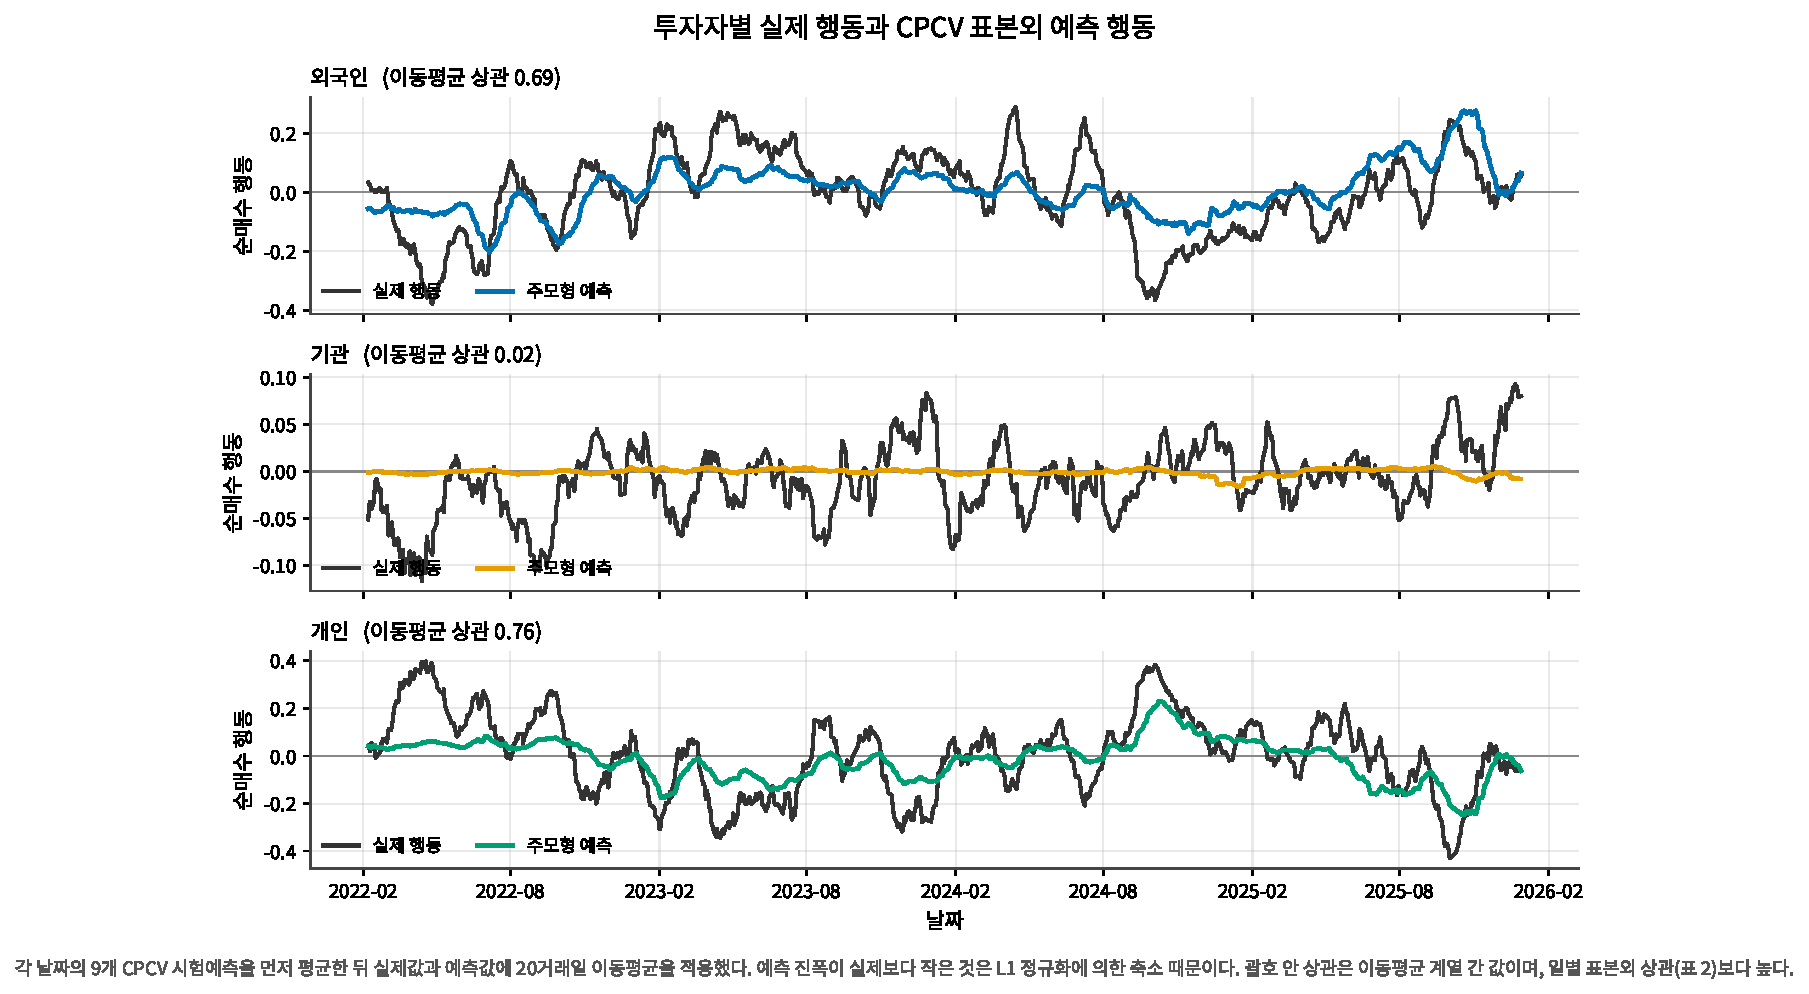
\includegraphics[width=\columnwidth]{figures/fig_actual_vs_prediction.pdf}
  \caption{Actual and out-of-sample predicted net buying (20-day moving average).
  The nine CPCV test predictions per date are averaged first. Correlations in the
  titles are between the smoothed series and are not directly comparable to the
  daily correlations in Table~\ref{tab:performance}.}
  \Description{Three line charts overlaying actual net buying and model
  predictions over time. In the institutional panel the prediction is flat near
  zero.}
  \label{fig:prediction}
\end{figure}

\begin{table}[t]
  \caption{Out-of-sample performance under CPCV (mean $\pm$ s.d.\ over 45
  splits) and the persistence baseline}
  \label{tab:performance}
  \small
  \centering
  \begin{tabular}{@{}lccc@{}}
    \toprule
    Metric & Foreign & Inst. & Retail \\
    \midrule
    \multicolumn{4}{@{}l}{\emph{SPR-IRL}}\\
    Directional accuracy & $0.636\pm0.039$ & $0.542\pm0.038$ & $0.608\pm0.044$ \\
    Correlation          & $0.278\pm0.110$ & $0.068\pm0.064$ & $0.245\pm0.118$ \\
    MAE                  & $0.195\pm0.019$ & $0.094\pm0.008$ & $0.264\pm0.029$ \\
    MAE / action s.d.    & $0.759$ & $0.756$ & $0.791$ \\
    Saturation rate      & $0.000$ & $0.000$ & $0.000$ \\
    \addlinespace
    \multicolumn{4}{@{}l}{\emph{Persistence} ($a_{t+1}\!\leftarrow\!a_t$)}\\
    Directional accuracy & $\mathbf{0.642}$ & $\mathbf{0.547}$ & $\mathbf{0.616}$ \\
    Correlation          & $\mathbf{0.359}$ & $\mathbf{0.136}$ & $\mathbf{0.311}$ \\
    \bottomrule
  \end{tabular}
\end{table}

In Figure~\ref{fig:prediction} the foreign and retail predictions track the
regime turns of the actual series (smoothed correlations 0.69 and 0.76) with a
smaller amplitude due to $L_1$ shrinkage, while the institutional prediction is
essentially pinned to zero (0.02).

Table~\ref{tab:performance} shows two things. First, dispersion across splits is
large, so types cannot be compared from a single split. Second, \textbf{the naive
persistence baseline beats SPR-IRL on directional accuracy and correlation}.
Since $a_t$ is published after the day-$t$ close this is an informationally
feasible rule. The reason is clear: the action has autocorrelation
$0.401/0.149/0.345$, yet the feature set contains no lagged own action.
Restricting the features to (F1)--(F3) was a design choice ensuring that all
types share only features corresponding to independently established
regularities, not a design for predictive performance.
Table~\ref{tab:performance} shows that the model has not merely fitted noise; it
is not evidence of predictive superiority.

Because the saturation rate is zero for every type and split, the premise of
Proposition~\ref{prop:lasso} holds and the estimator is literally a Lasso.

\subsection{Recovered Preferences: A Mirror Image}
\label{sec:beta}

\begin{figure*}[t]
  \centering
  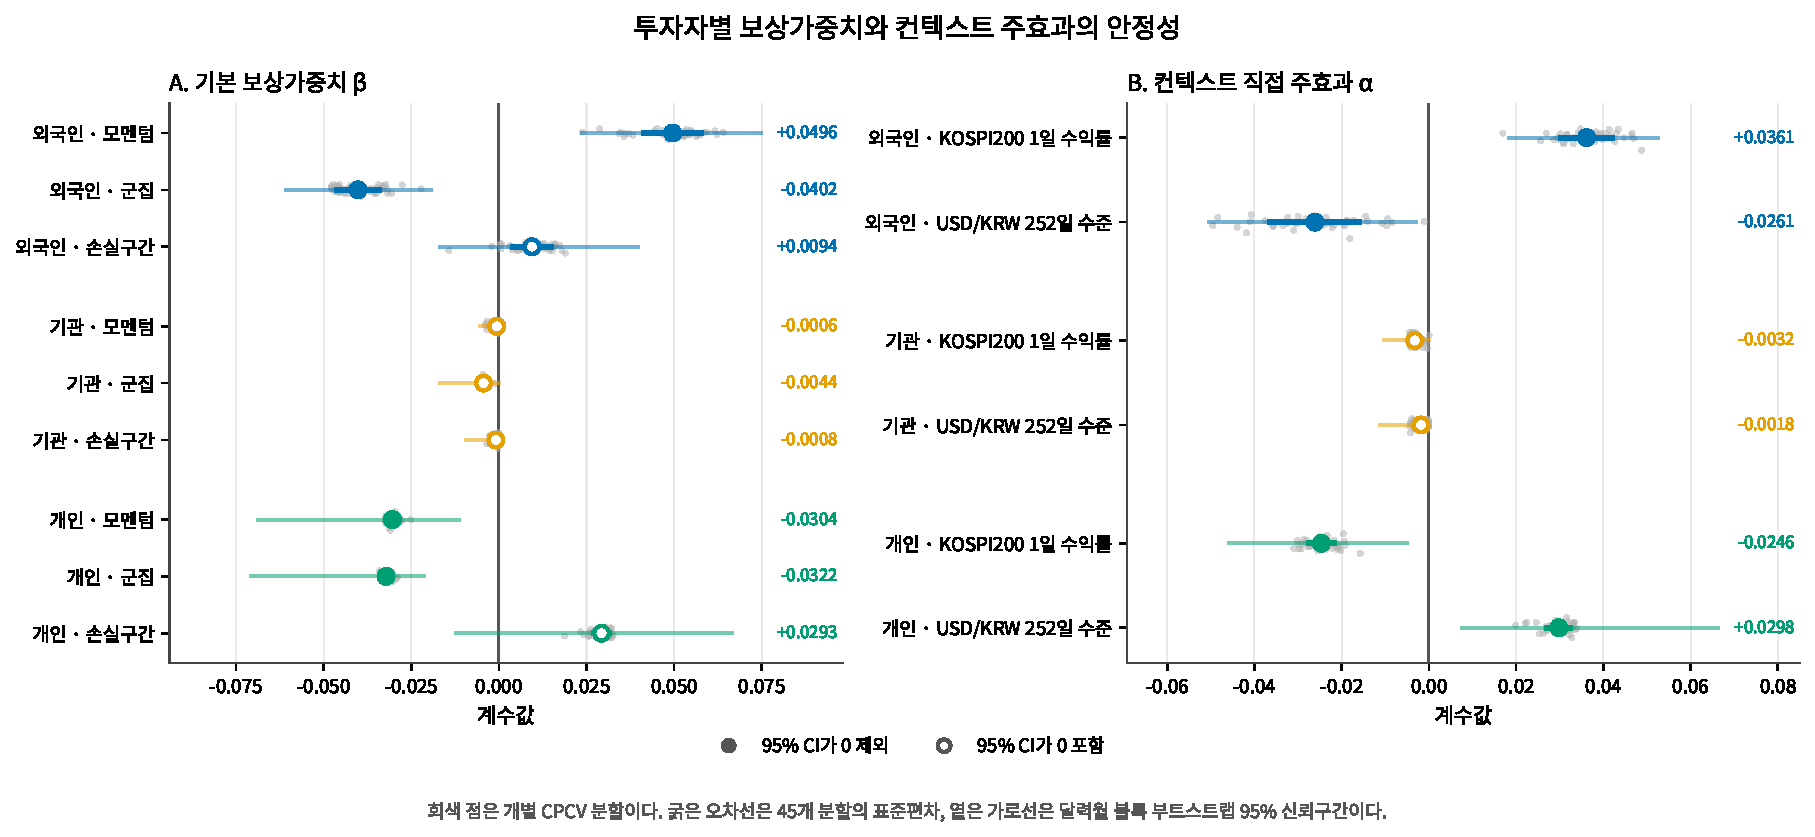
\includegraphics[width=\textwidth]{figures/fig_beta_alpha_forest.pdf}
  \caption{Stability of the recovered baseline reward weights $\beta$ (A) and
  context main effects $\alpha$ (B). Grey dots are the 45 individual CPCV splits,
  thick error bars the across-split standard deviation, and light horizontal
  lines the 95\% calendar-month block bootstrap interval. Hollow markers denote
  terms whose interval contains zero.}
  \Description{Two forest-plot panels. Panel A gives momentum, herding and
  underwater coefficients for the three types; panel B gives the KOSPI200 and FX
  main effects. Foreign momentum is positive, retail momentum negative, and every
  institutional marker is hollow.}
  \label{fig:forest}
\end{figure*}

\textbf{The mirror image on momentum.} The foreign momentum weight is $+0.0496$
and positive in all 45 splits; the retail weight is $-0.0304$ and negative in all
45. Their bootstrap intervals do not overlap and each excludes zero
(Figure~\ref{fig:forest}A). Although the same feature set was estimated
independently for each type, the two diverge in opposite directions, matching the
sign expectations of prior
work~\cite{grinblatt2000investment,choe1999foreign}.

\textbf{Reappearance in the context response.} The same mirror appears in the
main effects (Figure~\ref{fig:forest}B). Foreign investors move toward net buying
when the market rises ($+0.0361$) and toward net selling when the won is weak
($-0.0261$); retail investors do the opposite on both ($-0.0246$, $+0.0298$). All
four keep their sign in all 45 splits and all four intervals exclude zero.

\textbf{Herding.} The herding coefficient is negative in all 45 splits for all
three types, and the foreign ($-0.0402$) and retail ($-0.0322$) intervals exclude
zero. This does not separate a behavioural interpretation from the
market-clearing constraint: under the $-0.77$ same-day correlation of
\S\ref{sec:data}, much of the negative coefficient may be mechanical. We
therefore restrict the result to the descriptive statement that observed
aggregate flow shows a negative cross-type association, and the same reservation
applies to the mirrored main effects.

\textbf{Underwater.} The retail underwater weight is $+0.0293$ and positive in
all 45 splits, consistent with the reference-price dependence of the
disposition-effect
literature~\cite{shefrin1985disposition,odean1998investors}. However, as
Figure~\ref{fig:forest}A shows, the interval contains zero for all three types.
The retail interval is $[-0.0122,+0.0665]$: although the sign is 100\% consistent
across splits, it flips in 5.5\% of month-block resamples. This is precisely the
situation anticipated in \S\ref{sec:protocol}, where sign consistency understates
uncertainty because splits share observations. We therefore report a sign
consistent with the disposition effect without claiming it as established.

Of the twelve interaction coefficients, four keep their sign in all 45 splits
(foreign momentum $\times$ KOSPI200 $-0.0139$; retail momentum $\times$ FX
$+0.0144$; retail herding $\times$ KOSPI200 $-0.0080$; retail underwater $\times$
FX $-0.0186$), of which the first and last also pass the bootstrap. Since twelve
were examined jointly, we present them as exploratory only.

\subsection{Stability}
\label{sec:stability}

\begin{figure*}[t]
  \centering
  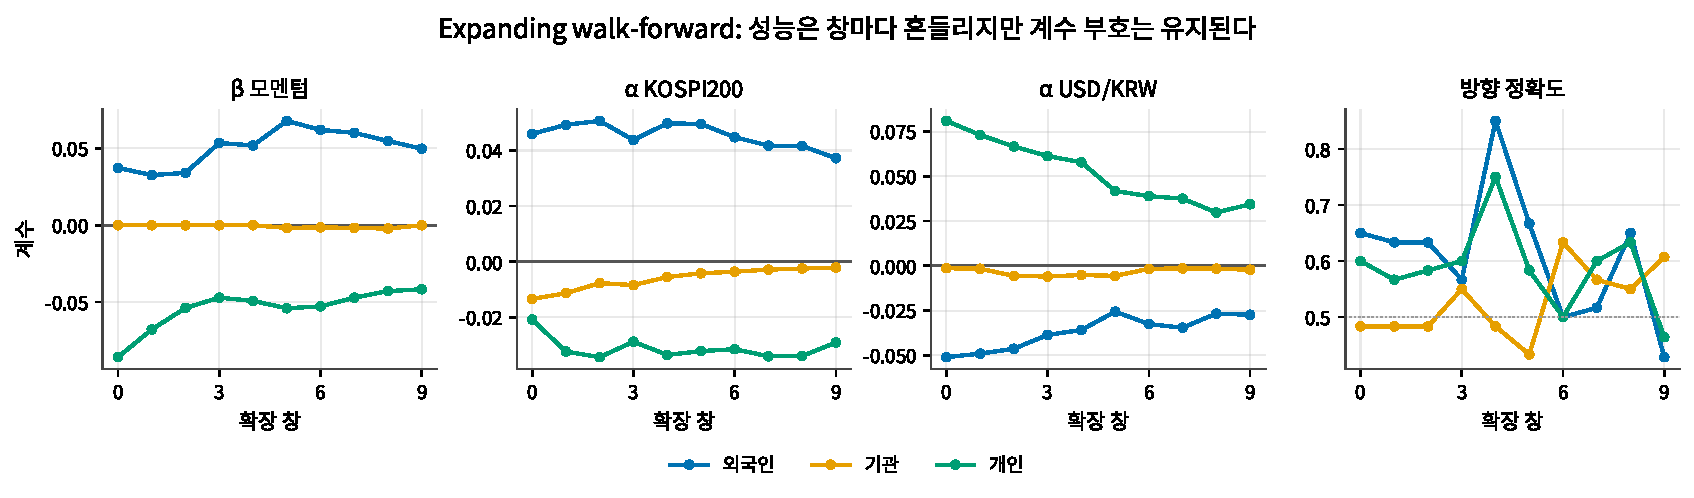
\includegraphics[width=\textwidth]{figures/fig_walk_forward.pdf}
  \caption{Coefficient paths and directional accuracy over ten expanding
  walk-forward windows. Performance fluctuates while the signs hold, and the
  foreign and retail momentum paths never cross.}
  \Description{Four line charts against the expanding-window index showing the
  momentum coefficient, two context main effects, and directional accuracy for
  the three types.}
  \label{fig:walkforward}
\end{figure*}

\textbf{(V2)} The bootstrap splits the results three ways: the eight terms
forming the momentum and context mirrors all exclude zero, the underwater weights
do not, and no institutional term does (the hollow markers in
Figure~\ref{fig:forest}).

\textbf{(V3)} In Figure~\ref{fig:walkforward} performance fluctuates sharply:
foreign directional accuracy moves between 0.43 and 0.85, averaging
$0.610\pm0.116$, and the correlation falls to $0.131\pm0.162$, less than half the
CPCV value of 0.278. Because CPCV can place a test fold ahead of a training fold
while walk-forward cannot, we report this degradation as a generalization limit
from the temporal structure. The coefficient paths, by contrast, do not
fluctuate: foreign momentum is positive in all ten windows and retail negative in
all ten, the two never cross, and the same mirror holds for both context main
effects. The institutional paths hug the zero line.

\textbf{(V4)} Foreign and retail coefficients agree to four decimal places under
$L_1$, $L_2$ and no penalty, so the mirror is not an artefact of the penalty.
Only the institutional coefficients move (herding
$-0.0076\rightarrow-0.0124$, underwater $-0.0000\rightarrow-0.0018$).

\subsection{Institutional Investors: A Converged Null}
\label{sec:null}

For institutional flow SPR-IRL finds no preference that is stably identified at
daily frequency, and we report this as a result. The evidence is fivefold:
(i) the prediction series degenerates to zero (Figure~\ref{fig:prediction});
(ii) excluding herding, the coefficients are about one fortieth of the other
types ($-0.0006$, $-0.0008$); (iii) no term excludes zero in the bootstrap
(Figure~\ref{fig:forest}); (iv) the coefficients depend on the choice of penalty;
and (v) momentum sign consistency is 40\% of ten walk-forward windows and
underwater 0\%.

\textbf{This null is not an optimization failure.} By
Proposition~\ref{prop:lasso}, Equation~\eqref{eq:loss} is convex with a unique
global optimum, and comparing the solution reached against the closed-form
optimum of the same objective leaves an institutional gap of only 0.17\% on
average and 0.48\% at most (0.21\% for foreign, 0.92\% for retail). All three
types reach the attainable optimum; only for institutional investors do the
coefficients there sit near zero. The data do not determine an institutional
preference; the optimizer did not fail to find one.

Economically this reads naturally: the ``institutional'' category aggregates
pension funds, investment trusts, insurers, private funds and securities firms,
so flows from agents with different objectives offset one another.

\subsection{Construct Validity}
\label{sec:construct}

\begin{table}[t]
  \caption{Prior sign expectations and recovered results}
  \label{tab:construct}
  \small
  \begin{tabular}{@{}>{\raggedright\arraybackslash}p{0.28\columnwidth}
                  >{\raggedright\arraybackslash}p{0.13\columnwidth}
                  >{\raggedright\arraybackslash}p{0.28\columnwidth}
                  >{\raggedright\arraybackslash}p{0.15\columnwidth}@{}}
    \toprule
    Regularity & Expected & Recovered & Verdict \\
    \midrule
    Foreign trend trading~\cite{grinblatt2000investment,choe1999foreign}
      & $\beta^{mom}\!>\!0$ & $+0.0496$ (100\%, CI excl.\ 0) & matches \\
    Retail contrarian~\cite{grinblatt2000investment,kaniel2008individual}
      & $\beta^{mom}\!<\!0$ & $-0.0304$ (100\%, CI excl.\ 0) & matches \\
    Disposition effect~\cite{shefrin1985disposition,odean1998investors}
      & $\beta^{uw}\!>\!0$ & $+0.0293$ (100\%, CI incl.\ 0) & partial \\
    Institutional herding~\cite{lakonishok1992impact}
      & $\beta^{herd}\!>\!0$ & $-0.0044$ (100\%, CI incl.\ 0) & mismatch \\
    \bottomrule
  \end{tabular}
\end{table}

Table~\ref{tab:construct} reports the contrast. That the recovered signs agree
with independently established regularities, and that two types diverge in
opposite directions on momentum, is evidence of construct validity given that
all types shared the same features and model form. The mismatch arises because
the measured object differs: Lakonishok et al.~\cite{lakonishok1992impact}
measure herding \emph{within} the institutional group, whereas
Equation~\eqref{eq:herd} measures whether institutions move with the
\emph{other two types}, so our result is not a refutation of that literature.

%  Packages: booktabs, graphicx, amsmath, array
%  Figures:  figures/  (three figures only)
%
%  Length target: Section 3 ~1.6 pp + Section 4 ~2.4 pp = ~4 pp,
%  leaving 3 pp for Sections 1-2 and 1 pp for Section 5 and references.
% =====================================================================

\section{Method: SPR-IRL}
\label{sec:method}

This section defines Symmetric Preference Recovery (SPR-IRL). SPR-IRL is not a
single model but a procedure comprising (i) symmetric estimation over shared
features, (ii) out-of-sample stability assessment, and (iii) a contrast against
sign expectations fixed in advance.

\subsection{Continuous Action and Symmetric Estimation}
\label{sec:setup}

Let the investor types be
$\mathcal{I}=\{\text{foreign},\text{institutional},\text{retail}\}$. Writing
$V^{buy}_{i,t}$ and $V^{sell}_{i,t}$ for the daily gross buy and sell value of
type $i$, the action is
\begin{equation}
u_{i,t}=\frac{V^{buy}_{i,t}-V^{sell}_{i,t}}
             {V^{buy}_{i,t}+V^{sell}_{i,t}}\in[-1,1].
\label{eq:action}
\end{equation}
Because the denominator is the type's own gross turnover rather than
market-wide turnover, $u_{i,t}$ is a common scale unaffected by differences in
trading size across types, and unlike a binary label it preserves intensity.

All three types receive the same state features $x_{i,t}\in\mathbb{R}^{3}$, the
same context $C_t\in\mathbb{R}^{2}$, and the same model form; only the
parameters $\theta_i=(\beta_i,B_i,\alpha_i)$ are estimated separately on each
type's own data. Since no type is assigned a different feature a priori, any
difference in the results is learned rather than imposed, and this is what
licenses direct comparison of coefficients across types.

The training sample is $(x_{i,t},C_t,a_{i,t+1})$ with $a_{i,t+1}=u_{i,t+1}$: a
day-$t$ state explains day-$t+1$ behaviour, so no future trade enters the
features.

\subsection{Reward Features and Market Context}
\label{sec:features}

All three features and both contexts are standardized on the training indices of
each split only, so every coefficient reads as the effect of a
one-standard-deviation move.

\textbf{(F1) Medium-term momentum} $x^{mom}_{t}=\log(P_t/P_{t-20})$. The 20-day
window is pre-specified for interpretability and was not tuned on the data. A
positive coefficient indicates trend following and a negative one contrarian
trading; the sign expectation follows the literature on type-specific momentum
trading~\cite{grinblatt2000investment,choe1999foreign}.

\textbf{(F2) Herding} is the cross-sectional average of the previous day's
actions of the two types other than $i$,
\begin{equation}
x^{herd}_{i,t}=\tfrac{1}{2}\left(u_{j,t-1}+u_{k,t-1}\right),\qquad j,k\neq i.
\label{eq:herd}
\end{equation}
The one-day lag is not an information constraint but a design choice that keeps
the same-day accounting offset between types out of the predictor set
(\S\ref{sec:beta}). The sign expectation follows the institutional herding
literature~\cite{lakonishok1992impact}, which however measures herding
\emph{within} the institutional group whereas Equation~\eqref{eq:herd} measures
a relation \emph{between} types.

\textbf{(F3) Underwater gap} uses an average-cost proxy $\bar P_{i,t}$ and the
day's gross-trade VWAP $P^{vwap}_{i,t}$,
\begin{equation}
x^{uw}_{i,t}=\max\!\left(
\frac{\bar P_{i,t}-P^{vwap}_{i,t}}{\bar P_{i,t}},\,0\right).
\label{eq:underwater}
\end{equation}
Truncation at zero makes the variable reference-point dependent by construction.
The average cost recursively updates an effective inventory from gross
quantities and values, multiplying the previous day's inventory by a forgetting
factor $\rho=0.98$ (half-life about 34 trading days). The sign expectation
follows the disposition-effect
literature~\cite{shefrin1985disposition,odean1998investors}. Because the proxy is
built from aggregate flow, the coefficient on $x^{uw}$ cannot be read as a direct
test of that effect.

\textbf{The context} consists of the one-day KOSPI200 return $r_t$ and the
KRW/USD level $z_t=(\log e_t-\mu_{t-1,252})/\sigma_{t-1,252}$, where the mean and
standard deviation use only data through $t-1$. Because Samsung Electronics
carries a large KOSPI200 weight, stock momentum overlaps the market return and
feature--context correlations range from $-0.29$ to $0.22$; individual
coefficients are therefore conditional associations given the other terms.

\subsection{Myopic Reward and the Reduction to Lasso}
\label{sec:model}

Define the action score of type $i$ as
\begin{equation}
q_{i,t}=(\beta_i+B_iC_t)^{\top}x_{i,t}+\alpha_i^{\top}C_t.
\label{eq:score}
\end{equation}
Here $\alpha$ is a level effect that shifts behaviour even at average features
and $B$ a slope effect that changes feature sensitivity across contexts.
Including interactions while omitting the lower-order term $C_t$ is a standard
specification error, so the inclusion of $\alpha$ is not something to justify
empirically. With the one-step reward
$R_i=q_{i,t}a-\tfrac{\kappa}{2}a^{2}$ the optimal policy is
\begin{equation}
a^{*}_{i,t+1}=\mathrm{clip}(q_{i,t}/\kappa,-1,1).
\label{eq:policy}
\end{equation}
Without the quadratic term the solution would be $\pm1$ almost always and
intensity could not be reproduced. We fix $\kappa=1$ for identification, which
normalizes the units of the reward and the coefficients rather than asserting
that the empirical curvature is one. The training objective is
\begin{equation}
\min_{\theta_i}\ \frac{1}{|\mathcal{D}_i|}
\sum_{t\in\mathcal{D}_i}\!\bigl(a^{*}_{i,t+1}-a_{i,t+1}\bigr)^{2}
+\lambda_i\lVert\theta_i\rVert_1,
\label{eq:loss}
\end{equation}
optimized independently per type with Adam~\cite{kingma2015adam}.

\begin{proposition}[Reduction to Lasso]
\label{prop:lasso}
Let
$z_{i,t}=[\,x_{i,t};\ \mathrm{vec}(x_{i,t}C_t^{\top});\ C_t\,]\in\mathbb{R}^{11}$
and $\theta_i=[\,\beta_i;\ \mathrm{vec}(B_i);\ \alpha_i\,]$, so that
$q_{i,t}=\theta_i^{\top}z_{i,t}$. If $|q_{i,t}|\le 1$ throughout the training
sample, the clip in Equation~\eqref{eq:policy} never binds, $a^{*}=q$, and
Equation~\eqref{eq:loss} becomes exactly an $L_1$-penalized (Lasso) regression of
$a_{i,t+1}$ on $z_{i,t}$.
\end{proposition}

In our sample the maximum $|q|$ is 0.842 for foreign, 0.587 for retail and 0.135
for institutional investors, and the saturation rate is exactly zero in all 45
splits, so the premise holds. In SPR-IRL, ``recovering a preference'' and
``regressing order flow'' are therefore numerically indistinguishable.

This is not a defect but a consequence of myopia. If the agent looks one step
ahead, today's action does not affect anything beyond tomorrow, so what the agent
wants (the reward) collapses onto what it does (the policy). Applying the
stochastic policy of maximum-entropy IRL~\cite{ziebart2008maximum},
$\pi\propto\exp(R/\tau)$, makes $\pi$ a truncated normal with mean $q$ whose
point estimate coincides with the above; the reduction is thus a property of the
myopic, quadratic-reward setting in general. The value of the IRL formulation
lies in the extension path: once state dynamics and multi-period value are
introduced, the reward separates from the policy and yields a structural recovery
that regression cannot reach (\S\ref{sec:discussion}).

\subsection{Validation Protocol}
\label{sec:protocol}

Rather than reporting the recovered coefficients as they are, we apply four
stages. \textbf{(V1)} Combinatorial purged
cross-validation~\cite{lopez2018advances} with ten temporal folds of which two
are test folds gives $\binom{10}{2}=45$ splits, with a one-day purge, a five-day
embargo, and all standardization fitted on training indices only. Because splits
share observations, sign consistency is interpreted as a stability indicator, not
a $p$-value. \textbf{(V2)} To address that limitation we partition the sample
into calendar-month blocks, resample 1{,}000 times, and obtain 95\% confidence
intervals; month blocks preserve the autocorrelation of daily flow within each
block. \textbf{(V3)} Because CPCV can place a test fold before a training fold,
we add an expanding walk-forward: train on the first 400 observations, predict
the next 60 trading days after a five-day purge, and repeat while expanding by 60
days, for ten windows. \textbf{(V4)} To confirm the results are not an artefact
of the $L_1$ penalty we re-estimate under $L_2$ and no penalty and compare signs.

Metrics are MAE, RMSE, directional accuracy (the fraction with
$\mathrm{sign}(a^{*})=\mathrm{sign}(a)$), the actual--predicted correlation, and
the saturation rate. Because action standard deviations differ across types,
absolute errors are not compared across types. As a naive reference we report a
persistence rule that predicts the previous day's own action.

% =====================================================================
\section{Experiments}
\label{sec:experiments}

\subsection{Data}
\label{sec:data}

From daily records for Samsung Electronics (005930) we use the most recent 973
rows for which the 252-day exchange-rate history, the 20-day momentum, and the
next day's action can all be computed; state dates run 2022-01-06 to 2025-12-29.
The single-stock design is not a sample limitation but a controlled setting that
removes stock fixed effects and liquidity differences and isolates preference
heterogeneity across types.

Mean actions are near zero for all three types, but standard deviations differ
(retail 0.334, foreign 0.257, institutional 0.125) and first-order
autocorrelations are 0.345, 0.401 and 0.149. Same-day actions across types are
strongly negatively related (foreign--retail $-0.772$, institutional--retail
$-0.499$), reflecting the market-clearing constraint that one type's buying must
appear as another's selling; this bounds the interpretation in \S\ref{sec:beta}.

Training settings are, per type, foreign 75 epochs / batch 256 / lr 0.001 /
$\lambda=0$; institutional 10 / 2048 / 0.0005 / 0.01; retail 20 / 512 / 0.001 /
0.0003, with seed 42, $\kappa=1$, and 11 parameters per type ($\beta$ 3, $B$ 6,
$\alpha$ 2).

\subsection{Out-of-Sample Behaviour Reproduction}
\label{sec:oos}

\begin{figure}[t]
  \centering
  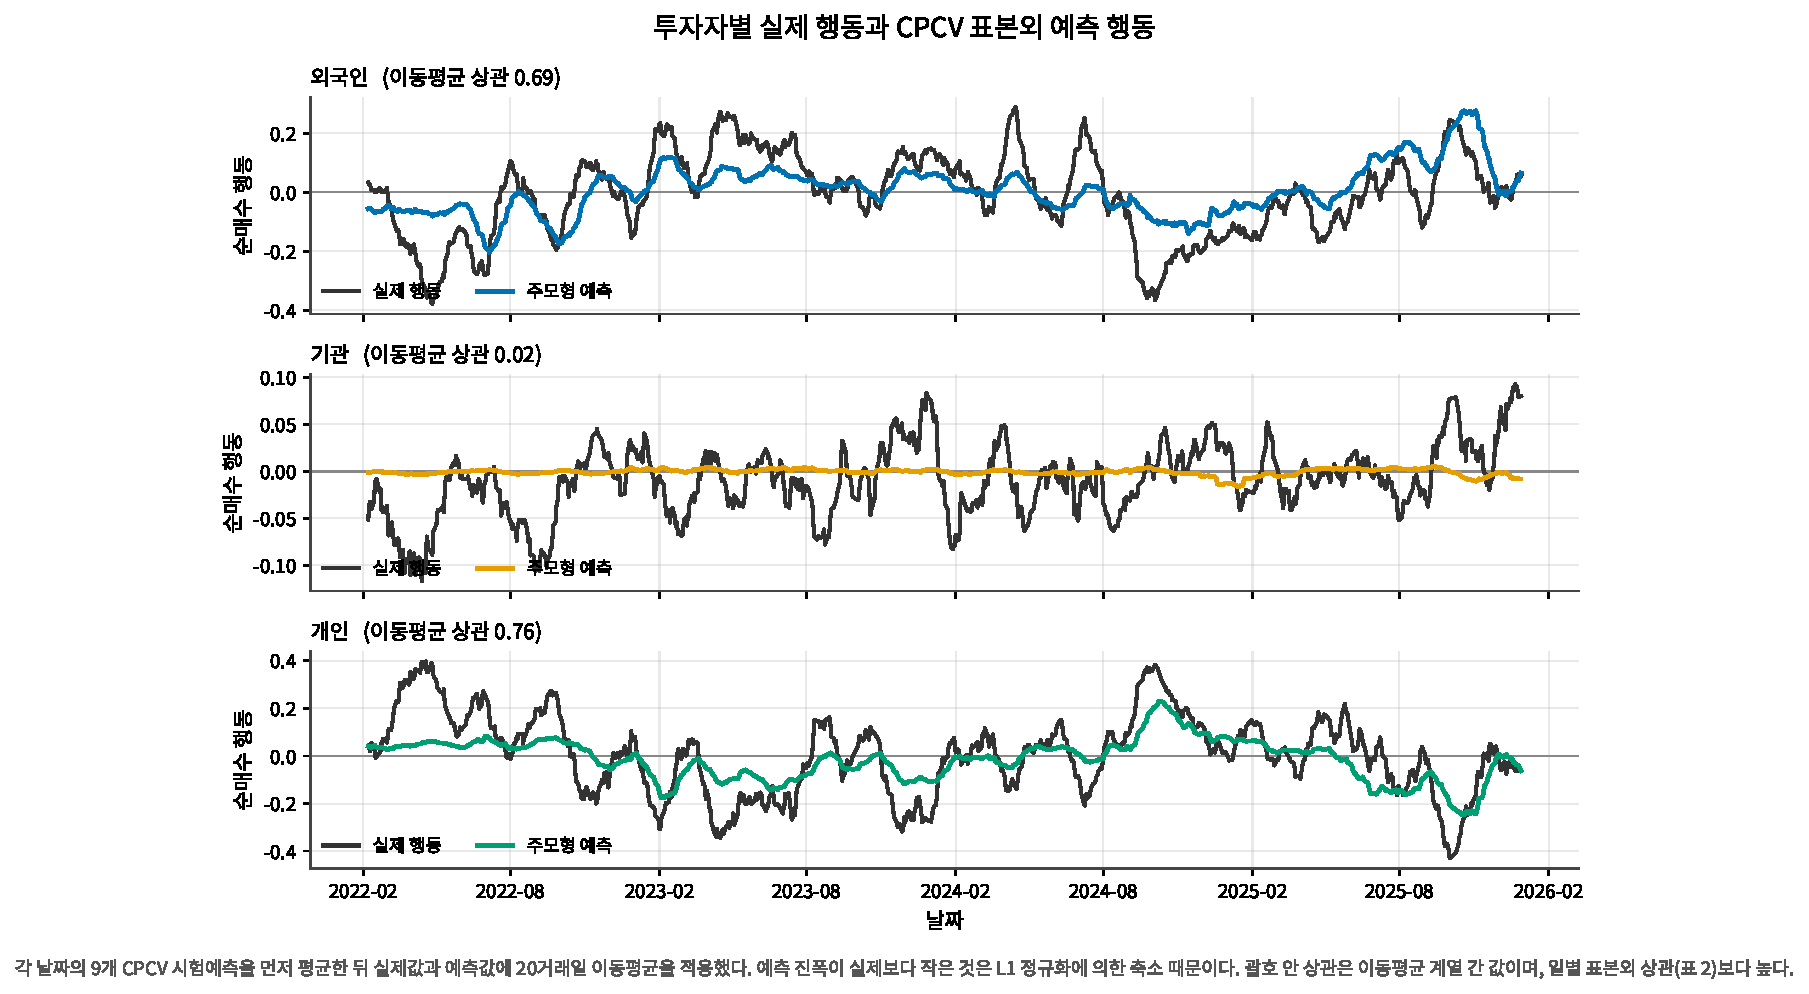
\includegraphics[width=\columnwidth]{figures/fig_actual_vs_prediction.pdf}
  \caption{Actual and out-of-sample predicted net buying (20-day moving average).
  The nine CPCV test predictions per date are averaged first. Correlations in the
  titles are between the smoothed series and are not directly comparable to the
  daily correlations in Table~\ref{tab:performance}.}
  \Description{Three line charts overlaying actual net buying and model
  predictions over time. In the institutional panel the prediction is flat near
  zero.}
  \label{fig:prediction}
\end{figure}

\begin{table}[t]
  \caption{Out-of-sample performance under CPCV (mean $\pm$ s.d.\ over 45
  splits) and the persistence baseline}
  \label{tab:performance}
  \small
  \centering
  \begin{tabular}{@{}lccc@{}}
    \toprule
    Metric & Foreign & Inst. & Retail \\
    \midrule
    \multicolumn{4}{@{}l}{\emph{SPR-IRL}}\\
    Directional accuracy & $0.636\pm0.039$ & $0.542\pm0.038$ & $0.608\pm0.044$ \\
    Correlation          & $0.278\pm0.110$ & $0.068\pm0.064$ & $0.245\pm0.118$ \\
    MAE                  & $0.195\pm0.019$ & $0.094\pm0.008$ & $0.264\pm0.029$ \\
    MAE / action s.d.    & $0.759$ & $0.756$ & $0.791$ \\
    Saturation rate      & $0.000$ & $0.000$ & $0.000$ \\
    \addlinespace
    \multicolumn{4}{@{}l}{\emph{Persistence} ($a_{t+1}\!\leftarrow\!a_t$)}\\
    Directional accuracy & $\mathbf{0.642}$ & $\mathbf{0.547}$ & $\mathbf{0.616}$ \\
    Correlation          & $\mathbf{0.359}$ & $\mathbf{0.136}$ & $\mathbf{0.311}$ \\
    \bottomrule
  \end{tabular}
\end{table}

In Figure~\ref{fig:prediction} the foreign and retail predictions track the
regime turns of the actual series (smoothed correlations 0.69 and 0.76) with a
smaller amplitude due to $L_1$ shrinkage, while the institutional prediction is
essentially pinned to zero (0.02).

Table~\ref{tab:performance} shows two things. First, dispersion across splits is
large, so types cannot be compared from a single split. Second, \textbf{the naive
persistence baseline beats SPR-IRL on directional accuracy and correlation}.
Since $a_t$ is published after the day-$t$ close this is an informationally
feasible rule. The reason is clear: the action has autocorrelation
$0.401/0.149/0.345$, yet the feature set contains no lagged own action.
Restricting the features to (F1)--(F3) was a design choice ensuring that all
types share only features corresponding to independently established
regularities, not a design for predictive performance.
Table~\ref{tab:performance} shows that the model has not merely fitted noise; it
is not evidence of predictive superiority.

Because the saturation rate is zero for every type and split, the premise of
Proposition~\ref{prop:lasso} holds and the estimator is literally a Lasso.

\subsection{Recovered Preferences: A Mirror Image}
\label{sec:beta}

\begin{figure*}[t]
  \centering
  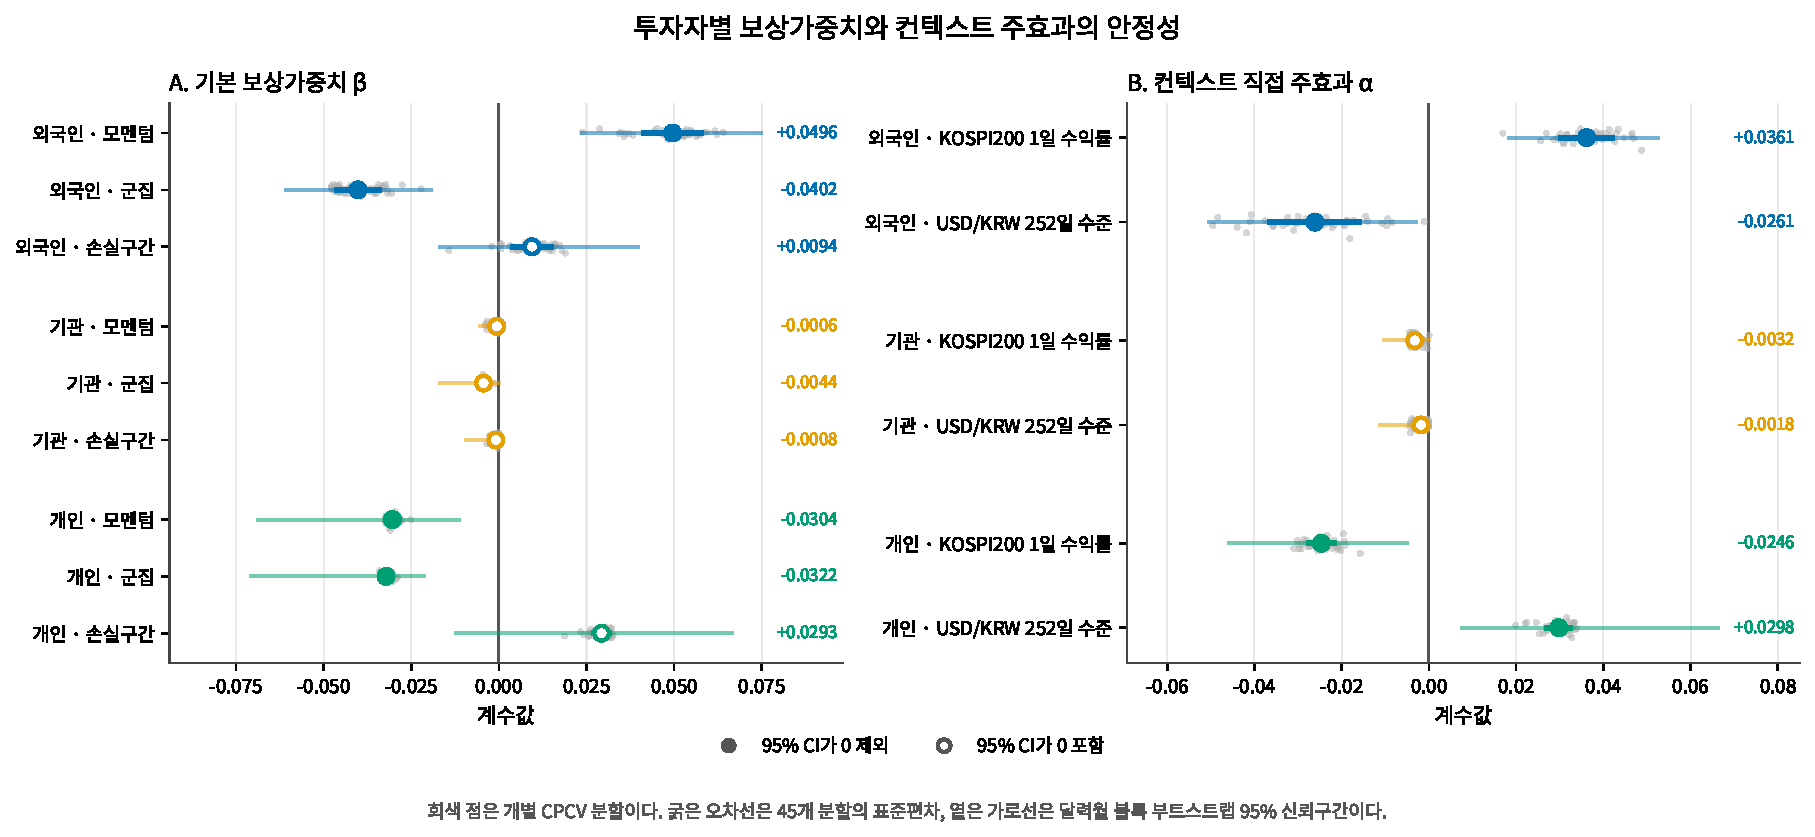
\includegraphics[width=\textwidth]{figures/fig_beta_alpha_forest.pdf}
  \caption{Stability of the recovered baseline reward weights $\beta$ (A) and
  context main effects $\alpha$ (B). Grey dots are the 45 individual CPCV splits,
  thick error bars the across-split standard deviation, and light horizontal
  lines the 95\% calendar-month block bootstrap interval. Hollow markers denote
  terms whose interval contains zero.}
  \Description{Two forest-plot panels. Panel A gives momentum, herding and
  underwater coefficients for the three types; panel B gives the KOSPI200 and FX
  main effects. Foreign momentum is positive, retail momentum negative, and every
  institutional marker is hollow.}
  \label{fig:forest}
\end{figure*}

\textbf{The mirror image on momentum.} The foreign momentum weight is $+0.0496$
and positive in all 45 splits; the retail weight is $-0.0304$ and negative in all
45. Their bootstrap intervals do not overlap and each excludes zero
(Figure~\ref{fig:forest}A). Although the same feature set was estimated
independently for each type, the two diverge in opposite directions, matching the
sign expectations of prior
work~\cite{grinblatt2000investment,choe1999foreign}.

\textbf{Reappearance in the context response.} The same mirror appears in the
main effects (Figure~\ref{fig:forest}B). Foreign investors move toward net buying
when the market rises ($+0.0361$) and toward net selling when the won is weak
($-0.0261$); retail investors do the opposite on both ($-0.0246$, $+0.0298$). All
four keep their sign in all 45 splits and all four intervals exclude zero.

\textbf{Herding.} The herding coefficient is negative in all 45 splits for all
three types, and the foreign ($-0.0402$) and retail ($-0.0322$) intervals exclude
zero. This does not separate a behavioural interpretation from the
market-clearing constraint: under the $-0.77$ same-day correlation of
\S\ref{sec:data}, much of the negative coefficient may be mechanical. We
therefore restrict the result to the descriptive statement that observed
aggregate flow shows a negative cross-type association, and the same reservation
applies to the mirrored main effects.

\textbf{Underwater.} The retail underwater weight is $+0.0293$ and positive in
all 45 splits, consistent with the reference-price dependence of the
disposition-effect
literature~\cite{shefrin1985disposition,odean1998investors}. However, as
Figure~\ref{fig:forest}A shows, the interval contains zero for all three types.
The retail interval is $[-0.0122,+0.0665]$: although the sign is 100\% consistent
across splits, it flips in 5.5\% of month-block resamples. This is precisely the
situation anticipated in \S\ref{sec:protocol}, where sign consistency understates
uncertainty because splits share observations. We therefore report a sign
consistent with the disposition effect without claiming it as established.

Of the twelve interaction coefficients, four keep their sign in all 45 splits
(foreign momentum $\times$ KOSPI200 $-0.0139$; retail momentum $\times$ FX
$+0.0144$; retail herding $\times$ KOSPI200 $-0.0080$; retail underwater $\times$
FX $-0.0186$), of which the first and last also pass the bootstrap. Since twelve
were examined jointly, we present them as exploratory only.

\subsection{Stability}
\label{sec:stability}

\begin{figure*}[t]
  \centering
  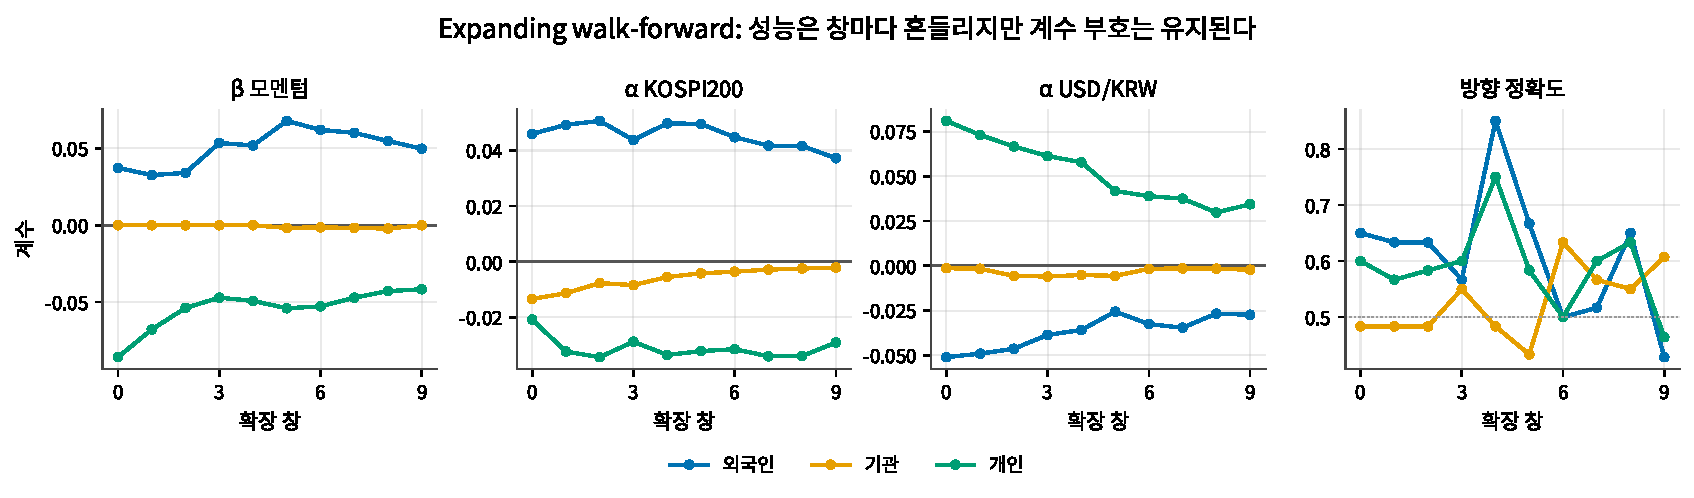
\includegraphics[width=\textwidth]{figures/fig_walk_forward.pdf}
  \caption{Coefficient paths and directional accuracy over ten expanding
  walk-forward windows. Performance fluctuates while the signs hold, and the
  foreign and retail momentum paths never cross.}
  \Description{Four line charts against the expanding-window index showing the
  momentum coefficient, two context main effects, and directional accuracy for
  the three types.}
  \label{fig:walkforward}
\end{figure*}

\textbf{(V2)} The bootstrap splits the results three ways: the eight terms
forming the momentum and context mirrors all exclude zero, the underwater weights
do not, and no institutional term does (the hollow markers in
Figure~\ref{fig:forest}).

\textbf{(V3)} In Figure~\ref{fig:walkforward} performance fluctuates sharply:
foreign directional accuracy moves between 0.43 and 0.85, averaging
$0.610\pm0.116$, and the correlation falls to $0.131\pm0.162$, less than half the
CPCV value of 0.278. Because CPCV can place a test fold ahead of a training fold
while walk-forward cannot, we report this degradation as a generalization limit
from the temporal structure. The coefficient paths, by contrast, do not
fluctuate: foreign momentum is positive in all ten windows and retail negative in
all ten, the two never cross, and the same mirror holds for both context main
effects. The institutional paths hug the zero line.

\textbf{(V4)} Foreign and retail coefficients agree to four decimal places under
$L_1$, $L_2$ and no penalty, so the mirror is not an artefact of the penalty.
Only the institutional coefficients move (herding
$-0.0076\rightarrow-0.0124$, underwater $-0.0000\rightarrow-0.0018$).

\subsection{Institutional Investors: A Converged Null}
\label{sec:null}

For institutional flow SPR-IRL finds no preference that is stably identified at
daily frequency, and we report this as a result. The evidence is fivefold:
(i) the prediction series degenerates to zero (Figure~\ref{fig:prediction});
(ii) excluding herding, the coefficients are about one fortieth of the other
types ($-0.0006$, $-0.0008$); (iii) no term excludes zero in the bootstrap
(Figure~\ref{fig:forest}); (iv) the coefficients depend on the choice of penalty;
and (v) momentum sign consistency is 40\% of ten walk-forward windows and
underwater 0\%.

\textbf{This null is not an optimization failure.} By
Proposition~\ref{prop:lasso}, Equation~\eqref{eq:loss} is convex with a unique
global optimum, and comparing the solution reached against the closed-form
optimum of the same objective leaves an institutional gap of only 0.17\% on
average and 0.48\% at most (0.21\% for foreign, 0.92\% for retail). All three
types reach the attainable optimum; only for institutional investors do the
coefficients there sit near zero. The data do not determine an institutional
preference; the optimizer did not fail to find one.

Economically this reads naturally: the ``institutional'' category aggregates
pension funds, investment trusts, insurers, private funds and securities firms,
so flows from agents with different objectives offset one another.

\subsection{Construct Validity}
\label{sec:construct}

\begin{table}[t]
  \caption{Prior sign expectations and recovered results}
  \label{tab:construct}
  \small
  \begin{tabular}{@{}>{\raggedright\arraybackslash}p{0.28\columnwidth}
                  >{\raggedright\arraybackslash}p{0.13\columnwidth}
                  >{\raggedright\arraybackslash}p{0.28\columnwidth}
                  >{\raggedright\arraybackslash}p{0.15\columnwidth}@{}}
    \toprule
    Regularity & Expected & Recovered & Verdict \\
    \midrule
    Foreign trend trading~\cite{grinblatt2000investment,choe1999foreign}
      & $\beta^{mom}\!>\!0$ & $+0.0496$ (100\%, CI excl.\ 0) & matches \\
    Retail contrarian~\cite{grinblatt2000investment,kaniel2008individual}
      & $\beta^{mom}\!<\!0$ & $-0.0304$ (100\%, CI excl.\ 0) & matches \\
    Disposition effect~\cite{shefrin1985disposition,odean1998investors}
      & $\beta^{uw}\!>\!0$ & $+0.0293$ (100\%, CI incl.\ 0) & partial \\
    Institutional herding~\cite{lakonishok1992impact}
      & $\beta^{herd}\!>\!0$ & $-0.0044$ (100\%, CI incl.\ 0) & mismatch \\
    \bottomrule
  \end{tabular}
\end{table}

Table~\ref{tab:construct} reports the contrast. That the recovered signs agree
with independently established regularities, and that two types diverge in
opposite directions on momentum, is evidence of construct validity given that
all types shared the same features and model form. The mismatch arises because
the measured object differs: Lakonishok et al.~\cite{lakonishok1992impact}
measure herding \emph{within} the institutional group, whereas
Equation~\eqref{eq:herd} measures whether institutions move with the
\emph{other two types}, so our result is not a refutation of that literature.

%  Packages: booktabs, graphicx, amsmath, array
%  Figures:  figures/  (three figures only)
%
%  Length target: Section 3 ~1.6 pp + Section 4 ~2.4 pp = ~4 pp,
%  leaving 3 pp for Sections 1-2 and 1 pp for Section 5 and references.
% =====================================================================

\section{Method: SPR-IRL}
\label{sec:method}

This section defines Symmetric Preference Recovery (SPR-IRL). SPR-IRL is not a
single model but a procedure comprising (i) symmetric estimation over shared
features, (ii) out-of-sample stability assessment, and (iii) a contrast against
sign expectations fixed in advance.

\subsection{Continuous Action and Symmetric Estimation}
\label{sec:setup}

Let the investor types be
$\mathcal{I}=\{\text{foreign},\text{institutional},\text{retail}\}$. Writing
$V^{buy}_{i,t}$ and $V^{sell}_{i,t}$ for the daily gross buy and sell value of
type $i$, the action is
\begin{equation}
u_{i,t}=\frac{V^{buy}_{i,t}-V^{sell}_{i,t}}
             {V^{buy}_{i,t}+V^{sell}_{i,t}}\in[-1,1].
\label{eq:action}
\end{equation}
Because the denominator is the type's own gross turnover rather than
market-wide turnover, $u_{i,t}$ is a common scale unaffected by differences in
trading size across types, and unlike a binary label it preserves intensity.

All three types receive the same state features $x_{i,t}\in\mathbb{R}^{3}$, the
same context $C_t\in\mathbb{R}^{2}$, and the same model form; only the
parameters $\theta_i=(\beta_i,B_i,\alpha_i)$ are estimated separately on each
type's own data. Since no type is assigned a different feature a priori, any
difference in the results is learned rather than imposed, and this is what
licenses direct comparison of coefficients across types.

The training sample is $(x_{i,t},C_t,a_{i,t+1})$ with $a_{i,t+1}=u_{i,t+1}$: a
day-$t$ state explains day-$t+1$ behaviour, so no future trade enters the
features.

\subsection{Reward Features and Market Context}
\label{sec:features}

All three features and both contexts are standardized on the training indices of
each split only, so every coefficient reads as the effect of a
one-standard-deviation move.

\textbf{(F1) Medium-term momentum} $x^{mom}_{t}=\log(P_t/P_{t-20})$. The 20-day
window is pre-specified for interpretability and was not tuned on the data. A
positive coefficient indicates trend following and a negative one contrarian
trading; the sign expectation follows the literature on type-specific momentum
trading~\cite{grinblatt2000investment,choe1999foreign}.

\textbf{(F2) Herding} is the cross-sectional average of the previous day's
actions of the two types other than $i$,
\begin{equation}
x^{herd}_{i,t}=\tfrac{1}{2}\left(u_{j,t-1}+u_{k,t-1}\right),\qquad j,k\neq i.
\label{eq:herd}
\end{equation}
The one-day lag is not an information constraint but a design choice that keeps
the same-day accounting offset between types out of the predictor set
(\S\ref{sec:beta}). The sign expectation follows the institutional herding
literature~\cite{lakonishok1992impact}, which however measures herding
\emph{within} the institutional group whereas Equation~\eqref{eq:herd} measures
a relation \emph{between} types.

\textbf{(F3) Underwater gap} uses an average-cost proxy $\bar P_{i,t}$ and the
day's gross-trade VWAP $P^{vwap}_{i,t}$,
\begin{equation}
x^{uw}_{i,t}=\max\!\left(
\frac{\bar P_{i,t}-P^{vwap}_{i,t}}{\bar P_{i,t}},\,0\right).
\label{eq:underwater}
\end{equation}
Truncation at zero makes the variable reference-point dependent by construction.
The average cost recursively updates an effective inventory from gross
quantities and values, multiplying the previous day's inventory by a forgetting
factor $\rho=0.98$ (half-life about 34 trading days). The sign expectation
follows the disposition-effect
literature~\cite{shefrin1985disposition,odean1998investors}. Because the proxy is
built from aggregate flow, the coefficient on $x^{uw}$ cannot be read as a direct
test of that effect.

\textbf{The context} consists of the one-day KOSPI200 return $r_t$ and the
KRW/USD level $z_t=(\log e_t-\mu_{t-1,252})/\sigma_{t-1,252}$, where the mean and
standard deviation use only data through $t-1$. Because Samsung Electronics
carries a large KOSPI200 weight, stock momentum overlaps the market return and
feature--context correlations range from $-0.29$ to $0.22$; individual
coefficients are therefore conditional associations given the other terms.

\subsection{Myopic Reward and the Reduction to Lasso}
\label{sec:model}

Define the action score of type $i$ as
\begin{equation}
q_{i,t}=(\beta_i+B_iC_t)^{\top}x_{i,t}+\alpha_i^{\top}C_t.
\label{eq:score}
\end{equation}
Here $\alpha$ is a level effect that shifts behaviour even at average features
and $B$ a slope effect that changes feature sensitivity across contexts.
Including interactions while omitting the lower-order term $C_t$ is a standard
specification error, so the inclusion of $\alpha$ is not something to justify
empirically. With the one-step reward
$R_i=q_{i,t}a-\tfrac{\kappa}{2}a^{2}$ the optimal policy is
\begin{equation}
a^{*}_{i,t+1}=\mathrm{clip}(q_{i,t}/\kappa,-1,1).
\label{eq:policy}
\end{equation}
Without the quadratic term the solution would be $\pm1$ almost always and
intensity could not be reproduced. We fix $\kappa=1$ for identification, which
normalizes the units of the reward and the coefficients rather than asserting
that the empirical curvature is one. The training objective is
\begin{equation}
\min_{\theta_i}\ \frac{1}{|\mathcal{D}_i|}
\sum_{t\in\mathcal{D}_i}\!\bigl(a^{*}_{i,t+1}-a_{i,t+1}\bigr)^{2}
+\lambda_i\lVert\theta_i\rVert_1,
\label{eq:loss}
\end{equation}
optimized independently per type with Adam~\cite{kingma2015adam}.

\begin{proposition}[Reduction to Lasso]
\label{prop:lasso}
Let
$z_{i,t}=[\,x_{i,t};\ \mathrm{vec}(x_{i,t}C_t^{\top});\ C_t\,]\in\mathbb{R}^{11}$
and $\theta_i=[\,\beta_i;\ \mathrm{vec}(B_i);\ \alpha_i\,]$, so that
$q_{i,t}=\theta_i^{\top}z_{i,t}$. If $|q_{i,t}|\le 1$ throughout the training
sample, the clip in Equation~\eqref{eq:policy} never binds, $a^{*}=q$, and
Equation~\eqref{eq:loss} becomes exactly an $L_1$-penalized (Lasso) regression of
$a_{i,t+1}$ on $z_{i,t}$.
\end{proposition}

In our sample the maximum $|q|$ is 0.842 for foreign, 0.587 for retail and 0.135
for institutional investors, and the saturation rate is exactly zero in all 45
splits, so the premise holds. In SPR-IRL, ``recovering a preference'' and
``regressing order flow'' are therefore numerically indistinguishable.

This is not a defect but a consequence of myopia. If the agent looks one step
ahead, today's action does not affect anything beyond tomorrow, so what the agent
wants (the reward) collapses onto what it does (the policy). Applying the
stochastic policy of maximum-entropy IRL~\cite{ziebart2008maximum},
$\pi\propto\exp(R/\tau)$, makes $\pi$ a truncated normal with mean $q$ whose
point estimate coincides with the above; the reduction is thus a property of the
myopic, quadratic-reward setting in general. The value of the IRL formulation
lies in the extension path: once state dynamics and multi-period value are
introduced, the reward separates from the policy and yields a structural recovery
that regression cannot reach (\S\ref{sec:discussion}).

\subsection{Validation Protocol}
\label{sec:protocol}

Rather than reporting the recovered coefficients as they are, we apply four
stages. \textbf{(V1)} Combinatorial purged
cross-validation~\cite{lopez2018advances} with ten temporal folds of which two
are test folds gives $\binom{10}{2}=45$ splits, with a one-day purge, a five-day
embargo, and all standardization fitted on training indices only. Because splits
share observations, sign consistency is interpreted as a stability indicator, not
a $p$-value. \textbf{(V2)} To address that limitation we partition the sample
into calendar-month blocks, resample 1{,}000 times, and obtain 95\% confidence
intervals; month blocks preserve the autocorrelation of daily flow within each
block. \textbf{(V3)} Because CPCV can place a test fold before a training fold,
we add an expanding walk-forward: train on the first 400 observations, predict
the next 60 trading days after a five-day purge, and repeat while expanding by 60
days, for ten windows. \textbf{(V4)} To confirm the results are not an artefact
of the $L_1$ penalty we re-estimate under $L_2$ and no penalty and compare signs.

Metrics are MAE, RMSE, directional accuracy (the fraction with
$\mathrm{sign}(a^{*})=\mathrm{sign}(a)$), the actual--predicted correlation, and
the saturation rate. Because action standard deviations differ across types,
absolute errors are not compared across types. As a naive reference we report a
persistence rule that predicts the previous day's own action.

% =====================================================================
\section{Experiments}
\label{sec:experiments}

\subsection{Data}
\label{sec:data}

From daily records for Samsung Electronics (005930) we use the most recent 973
rows for which the 252-day exchange-rate history, the 20-day momentum, and the
next day's action can all be computed; state dates run 2022-01-06 to 2025-12-29.
The single-stock design is not a sample limitation but a controlled setting that
removes stock fixed effects and liquidity differences and isolates preference
heterogeneity across types.

Mean actions are near zero for all three types, but standard deviations differ
(retail 0.334, foreign 0.257, institutional 0.125) and first-order
autocorrelations are 0.345, 0.401 and 0.149. Same-day actions across types are
strongly negatively related (foreign--retail $-0.772$, institutional--retail
$-0.499$), reflecting the market-clearing constraint that one type's buying must
appear as another's selling; this bounds the interpretation in \S\ref{sec:beta}.

Training settings are, per type, foreign 75 epochs / batch 256 / lr 0.001 /
$\lambda=0$; institutional 10 / 2048 / 0.0005 / 0.01; retail 20 / 512 / 0.001 /
0.0003, with seed 42, $\kappa=1$, and 11 parameters per type ($\beta$ 3, $B$ 6,
$\alpha$ 2).

\subsection{Out-of-Sample Behaviour Reproduction}
\label{sec:oos}

\begin{figure}[t]
  \centering
  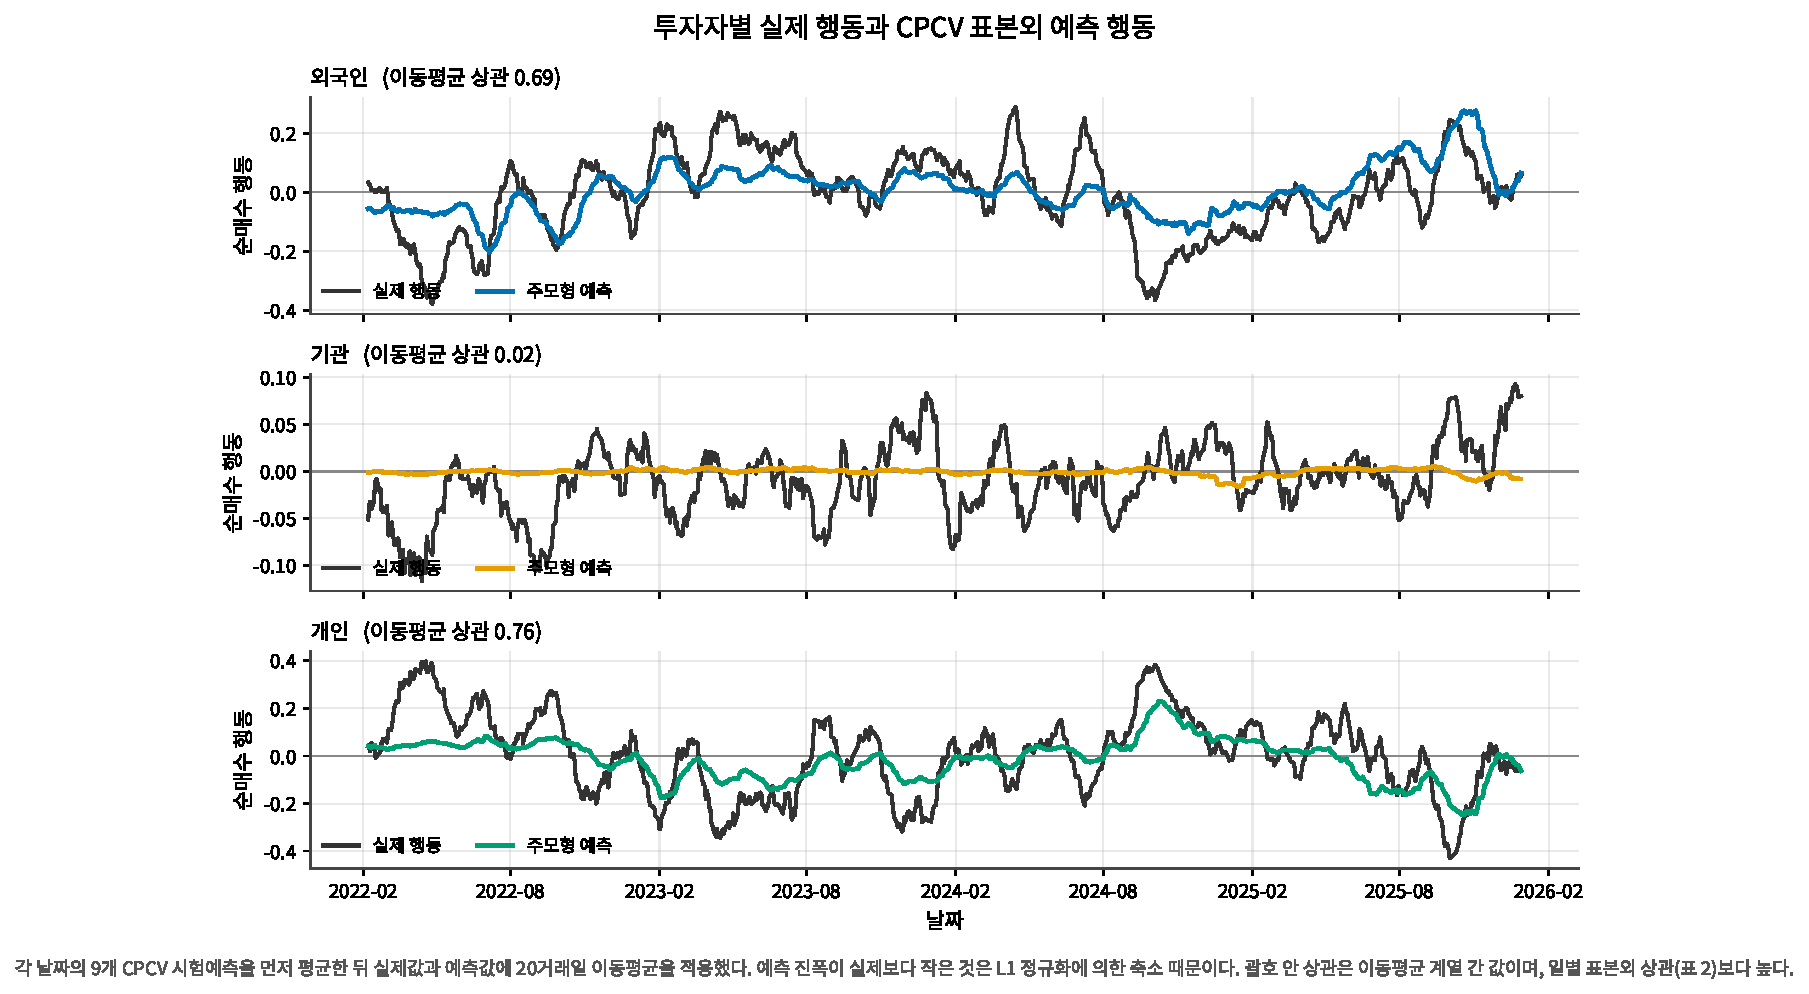
\includegraphics[width=\columnwidth]{figures/fig_actual_vs_prediction.pdf}
  \caption{Actual and out-of-sample predicted net buying (20-day moving average).
  The nine CPCV test predictions per date are averaged first. Correlations in the
  titles are between the smoothed series and are not directly comparable to the
  daily correlations in Table~\ref{tab:performance}.}
  \Description{Three line charts overlaying actual net buying and model
  predictions over time. In the institutional panel the prediction is flat near
  zero.}
  \label{fig:prediction}
\end{figure}

\begin{table}[t]
  \caption{Out-of-sample performance under CPCV (mean $\pm$ s.d.\ over 45
  splits) and the persistence baseline}
  \label{tab:performance}
  \small
  \centering
  \begin{tabular}{@{}lccc@{}}
    \toprule
    Metric & Foreign & Inst. & Retail \\
    \midrule
    \multicolumn{4}{@{}l}{\emph{SPR-IRL}}\\
    Directional accuracy & $0.636\pm0.039$ & $0.542\pm0.038$ & $0.608\pm0.044$ \\
    Correlation          & $0.278\pm0.110$ & $0.068\pm0.064$ & $0.245\pm0.118$ \\
    MAE                  & $0.195\pm0.019$ & $0.094\pm0.008$ & $0.264\pm0.029$ \\
    MAE / action s.d.    & $0.759$ & $0.756$ & $0.791$ \\
    Saturation rate      & $0.000$ & $0.000$ & $0.000$ \\
    \addlinespace
    \multicolumn{4}{@{}l}{\emph{Persistence} ($a_{t+1}\!\leftarrow\!a_t$)}\\
    Directional accuracy & $\mathbf{0.642}$ & $\mathbf{0.547}$ & $\mathbf{0.616}$ \\
    Correlation          & $\mathbf{0.359}$ & $\mathbf{0.136}$ & $\mathbf{0.311}$ \\
    \bottomrule
  \end{tabular}
\end{table}

In Figure~\ref{fig:prediction} the foreign and retail predictions track the
regime turns of the actual series (smoothed correlations 0.69 and 0.76) with a
smaller amplitude due to $L_1$ shrinkage, while the institutional prediction is
essentially pinned to zero (0.02).

Table~\ref{tab:performance} shows two things. First, dispersion across splits is
large, so types cannot be compared from a single split. Second, \textbf{the naive
persistence baseline beats SPR-IRL on directional accuracy and correlation}.
Since $a_t$ is published after the day-$t$ close this is an informationally
feasible rule. The reason is clear: the action has autocorrelation
$0.401/0.149/0.345$, yet the feature set contains no lagged own action.
Restricting the features to (F1)--(F3) was a design choice ensuring that all
types share only features corresponding to independently established
regularities, not a design for predictive performance.
Table~\ref{tab:performance} shows that the model has not merely fitted noise; it
is not evidence of predictive superiority.

Because the saturation rate is zero for every type and split, the premise of
Proposition~\ref{prop:lasso} holds and the estimator is literally a Lasso.

\subsection{Recovered Preferences: A Mirror Image}
\label{sec:beta}

\begin{figure*}[t]
  \centering
  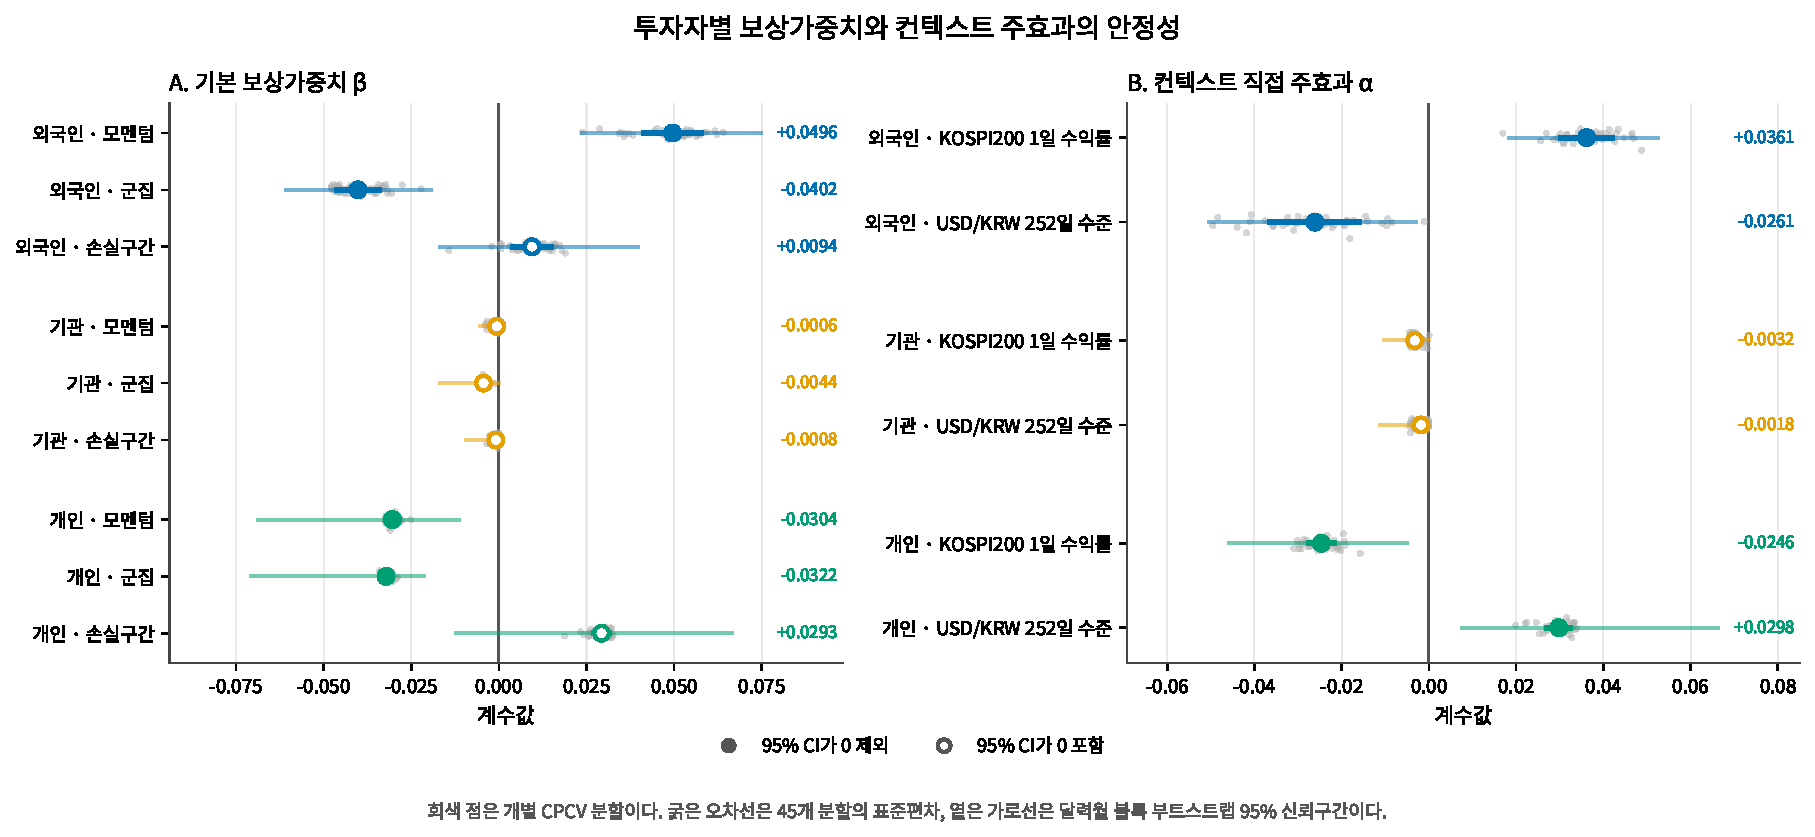
\includegraphics[width=\textwidth]{figures/fig_beta_alpha_forest.pdf}
  \caption{Stability of the recovered baseline reward weights $\beta$ (A) and
  context main effects $\alpha$ (B). Grey dots are the 45 individual CPCV splits,
  thick error bars the across-split standard deviation, and light horizontal
  lines the 95\% calendar-month block bootstrap interval. Hollow markers denote
  terms whose interval contains zero.}
  \Description{Two forest-plot panels. Panel A gives momentum, herding and
  underwater coefficients for the three types; panel B gives the KOSPI200 and FX
  main effects. Foreign momentum is positive, retail momentum negative, and every
  institutional marker is hollow.}
  \label{fig:forest}
\end{figure*}

\textbf{The mirror image on momentum.} The foreign momentum weight is $+0.0496$
and positive in all 45 splits; the retail weight is $-0.0304$ and negative in all
45. Their bootstrap intervals do not overlap and each excludes zero
(Figure~\ref{fig:forest}A). Although the same feature set was estimated
independently for each type, the two diverge in opposite directions, matching the
sign expectations of prior
work~\cite{grinblatt2000investment,choe1999foreign}.

\textbf{Reappearance in the context response.} The same mirror appears in the
main effects (Figure~\ref{fig:forest}B). Foreign investors move toward net buying
when the market rises ($+0.0361$) and toward net selling when the won is weak
($-0.0261$); retail investors do the opposite on both ($-0.0246$, $+0.0298$). All
four keep their sign in all 45 splits and all four intervals exclude zero.

\textbf{Herding.} The herding coefficient is negative in all 45 splits for all
three types, and the foreign ($-0.0402$) and retail ($-0.0322$) intervals exclude
zero. This does not separate a behavioural interpretation from the
market-clearing constraint: under the $-0.77$ same-day correlation of
\S\ref{sec:data}, much of the negative coefficient may be mechanical. We
therefore restrict the result to the descriptive statement that observed
aggregate flow shows a negative cross-type association, and the same reservation
applies to the mirrored main effects.

\textbf{Underwater.} The retail underwater weight is $+0.0293$ and positive in
all 45 splits, consistent with the reference-price dependence of the
disposition-effect
literature~\cite{shefrin1985disposition,odean1998investors}. However, as
Figure~\ref{fig:forest}A shows, the interval contains zero for all three types.
The retail interval is $[-0.0122,+0.0665]$: although the sign is 100\% consistent
across splits, it flips in 5.5\% of month-block resamples. This is precisely the
situation anticipated in \S\ref{sec:protocol}, where sign consistency understates
uncertainty because splits share observations. We therefore report a sign
consistent with the disposition effect without claiming it as established.

Of the twelve interaction coefficients, four keep their sign in all 45 splits
(foreign momentum $\times$ KOSPI200 $-0.0139$; retail momentum $\times$ FX
$+0.0144$; retail herding $\times$ KOSPI200 $-0.0080$; retail underwater $\times$
FX $-0.0186$), of which the first and last also pass the bootstrap. Since twelve
were examined jointly, we present them as exploratory only.

\subsection{Stability}
\label{sec:stability}

\begin{figure*}[t]
  \centering
  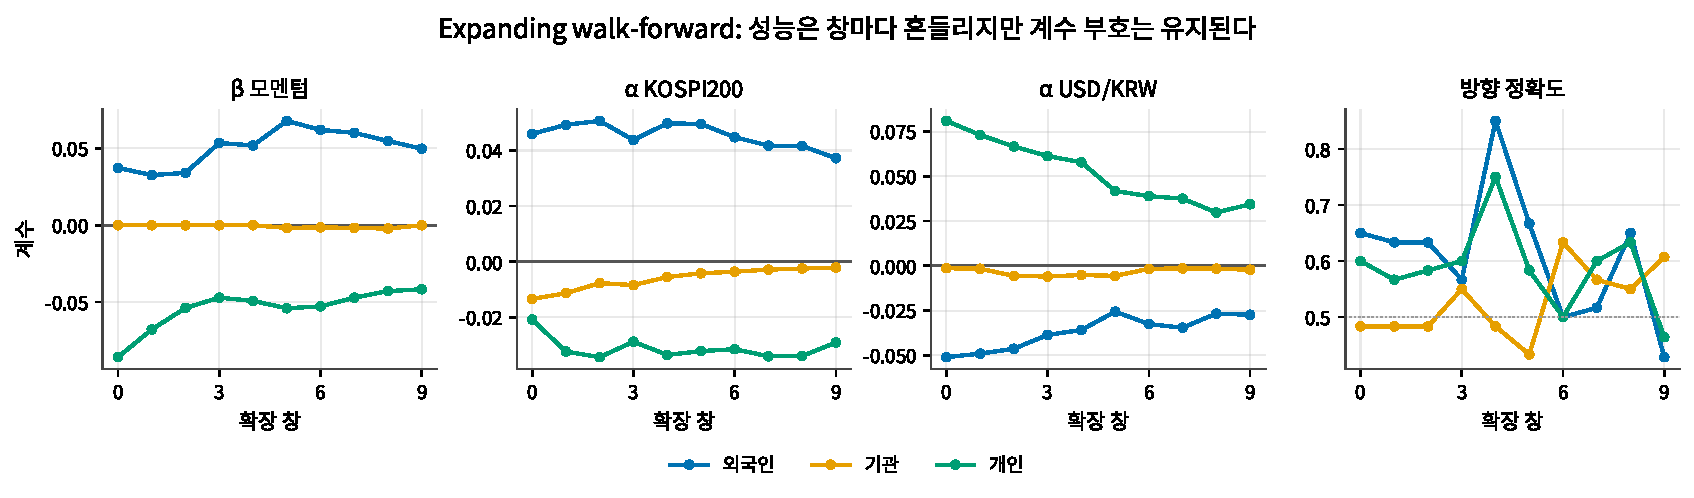
\includegraphics[width=\textwidth]{figures/fig_walk_forward.pdf}
  \caption{Coefficient paths and directional accuracy over ten expanding
  walk-forward windows. Performance fluctuates while the signs hold, and the
  foreign and retail momentum paths never cross.}
  \Description{Four line charts against the expanding-window index showing the
  momentum coefficient, two context main effects, and directional accuracy for
  the three types.}
  \label{fig:walkforward}
\end{figure*}

\textbf{(V2)} The bootstrap splits the results three ways: the eight terms
forming the momentum and context mirrors all exclude zero, the underwater weights
do not, and no institutional term does (the hollow markers in
Figure~\ref{fig:forest}).

\textbf{(V3)} In Figure~\ref{fig:walkforward} performance fluctuates sharply:
foreign directional accuracy moves between 0.43 and 0.85, averaging
$0.610\pm0.116$, and the correlation falls to $0.131\pm0.162$, less than half the
CPCV value of 0.278. Because CPCV can place a test fold ahead of a training fold
while walk-forward cannot, we report this degradation as a generalization limit
from the temporal structure. The coefficient paths, by contrast, do not
fluctuate: foreign momentum is positive in all ten windows and retail negative in
all ten, the two never cross, and the same mirror holds for both context main
effects. The institutional paths hug the zero line.

\textbf{(V4)} Foreign and retail coefficients agree to four decimal places under
$L_1$, $L_2$ and no penalty, so the mirror is not an artefact of the penalty.
Only the institutional coefficients move (herding
$-0.0076\rightarrow-0.0124$, underwater $-0.0000\rightarrow-0.0018$).

\subsection{Institutional Investors: A Converged Null}
\label{sec:null}

For institutional flow SPR-IRL finds no preference that is stably identified at
daily frequency, and we report this as a result. The evidence is fivefold:
(i) the prediction series degenerates to zero (Figure~\ref{fig:prediction});
(ii) excluding herding, the coefficients are about one fortieth of the other
types ($-0.0006$, $-0.0008$); (iii) no term excludes zero in the bootstrap
(Figure~\ref{fig:forest}); (iv) the coefficients depend on the choice of penalty;
and (v) momentum sign consistency is 40\% of ten walk-forward windows and
underwater 0\%.

\textbf{This null is not an optimization failure.} By
Proposition~\ref{prop:lasso}, Equation~\eqref{eq:loss} is convex with a unique
global optimum, and comparing the solution reached against the closed-form
optimum of the same objective leaves an institutional gap of only 0.17\% on
average and 0.48\% at most (0.21\% for foreign, 0.92\% for retail). All three
types reach the attainable optimum; only for institutional investors do the
coefficients there sit near zero. The data do not determine an institutional
preference; the optimizer did not fail to find one.

Economically this reads naturally: the ``institutional'' category aggregates
pension funds, investment trusts, insurers, private funds and securities firms,
so flows from agents with different objectives offset one another.

\subsection{Construct Validity}
\label{sec:construct}

\begin{table}[t]
  \caption{Prior sign expectations and recovered results}
  \label{tab:construct}
  \small
  \begin{tabular}{@{}>{\raggedright\arraybackslash}p{0.28\columnwidth}
                  >{\raggedright\arraybackslash}p{0.13\columnwidth}
                  >{\raggedright\arraybackslash}p{0.28\columnwidth}
                  >{\raggedright\arraybackslash}p{0.15\columnwidth}@{}}
    \toprule
    Regularity & Expected & Recovered & Verdict \\
    \midrule
    Foreign trend trading~\cite{grinblatt2000investment,choe1999foreign}
      & $\beta^{mom}\!>\!0$ & $+0.0496$ (100\%, CI excl.\ 0) & matches \\
    Retail contrarian~\cite{grinblatt2000investment,kaniel2008individual}
      & $\beta^{mom}\!<\!0$ & $-0.0304$ (100\%, CI excl.\ 0) & matches \\
    Disposition effect~\cite{shefrin1985disposition,odean1998investors}
      & $\beta^{uw}\!>\!0$ & $+0.0293$ (100\%, CI incl.\ 0) & partial \\
    Institutional herding~\cite{lakonishok1992impact}
      & $\beta^{herd}\!>\!0$ & $-0.0044$ (100\%, CI incl.\ 0) & mismatch \\
    \bottomrule
  \end{tabular}
\end{table}

Table~\ref{tab:construct} reports the contrast. That the recovered signs agree
with independently established regularities, and that two types diverge in
opposite directions on momentum, is evidence of construct validity given that
all types shared the same features and model form. The mismatch arises because
the measured object differs: Lakonishok et al.~\cite{lakonishok1992impact}
measure herding \emph{within} the institutional group, whereas
Equation~\eqref{eq:herd} measures whether institutions move with the
\emph{other two types}, so our result is not a refutation of that literature.

%  Packages: booktabs, graphicx, amsmath, array
%  Figures:  figures/  (three figures only)
%
%  Length target: Section 3 ~1.6 pp + Section 4 ~2.4 pp = ~4 pp,
%  leaving 3 pp for Sections 1-2 and 1 pp for Section 5 and references.
% =====================================================================

\section{Method: SPR-IRL}
\label{sec:method}

This section defines Symmetric Preference Recovery (SPR-IRL). SPR-IRL is not a
single model but a procedure comprising (i) symmetric estimation over shared
features, (ii) out-of-sample stability assessment, and (iii) a contrast against
sign expectations fixed in advance.

\subsection{Continuous Action and Symmetric Estimation}
\label{sec:setup}

Let the investor types be
$\mathcal{I}=\{\text{foreign},\text{institutional},\text{retail}\}$. Writing
$V^{buy}_{i,t}$ and $V^{sell}_{i,t}$ for the daily gross buy and sell value of
type $i$, the action is
\begin{equation}
u_{i,t}=\frac{V^{buy}_{i,t}-V^{sell}_{i,t}}
             {V^{buy}_{i,t}+V^{sell}_{i,t}}\in[-1,1].
\label{eq:action}
\end{equation}
Because the denominator is the type's own gross turnover rather than
market-wide turnover, $u_{i,t}$ is a common scale unaffected by differences in
trading size across types, and unlike a binary label it preserves intensity.

All three types receive the same state features $x_{i,t}\in\mathbb{R}^{3}$, the
same context $C_t\in\mathbb{R}^{2}$, and the same model form; only the
parameters $\theta_i=(\beta_i,B_i,\alpha_i)$ are estimated separately on each
type's own data. Since no type is assigned a different feature a priori, any
difference in the results is learned rather than imposed, and this is what
licenses direct comparison of coefficients across types.

The training sample is $(x_{i,t},C_t,a_{i,t+1})$ with $a_{i,t+1}=u_{i,t+1}$: a
day-$t$ state explains day-$t+1$ behaviour, so no future trade enters the
features.

\subsection{Reward Features and Market Context}
\label{sec:features}

All three features and both contexts are standardized on the training indices of
each split only, so every coefficient reads as the effect of a
one-standard-deviation move.

\textbf{(F1) Medium-term momentum} $x^{mom}_{t}=\log(P_t/P_{t-20})$. The 20-day
window is pre-specified for interpretability and was not tuned on the data. A
positive coefficient indicates trend following and a negative one contrarian
trading; the sign expectation follows the literature on type-specific momentum
trading~\cite{grinblatt2000investment,choe1999foreign}.

\textbf{(F2) Herding} is the cross-sectional average of the previous day's
actions of the two types other than $i$,
\begin{equation}
x^{herd}_{i,t}=\tfrac{1}{2}\left(u_{j,t-1}+u_{k,t-1}\right),\qquad j,k\neq i.
\label{eq:herd}
\end{equation}
The one-day lag is not an information constraint but a design choice that keeps
the same-day accounting offset between types out of the predictor set
(\S\ref{sec:beta}). The sign expectation follows the institutional herding
literature~\cite{lakonishok1992impact}, which however measures herding
\emph{within} the institutional group whereas Equation~\eqref{eq:herd} measures
a relation \emph{between} types.

\textbf{(F3) Underwater gap} uses an average-cost proxy $\bar P_{i,t}$ and the
day's gross-trade VWAP $P^{vwap}_{i,t}$,
\begin{equation}
x^{uw}_{i,t}=\max\!\left(
\frac{\bar P_{i,t}-P^{vwap}_{i,t}}{\bar P_{i,t}},\,0\right).
\label{eq:underwater}
\end{equation}
Truncation at zero makes the variable reference-point dependent by construction.
The average cost recursively updates an effective inventory from gross
quantities and values, multiplying the previous day's inventory by a forgetting
factor $\rho=0.98$ (half-life about 34 trading days). The sign expectation
follows the disposition-effect
literature~\cite{shefrin1985disposition,odean1998investors}. Because the proxy is
built from aggregate flow, the coefficient on $x^{uw}$ cannot be read as a direct
test of that effect.

\textbf{The context} consists of the one-day KOSPI200 return $r_t$ and the
KRW/USD level $z_t=(\log e_t-\mu_{t-1,252})/\sigma_{t-1,252}$, where the mean and
standard deviation use only data through $t-1$. Because Samsung Electronics
carries a large KOSPI200 weight, stock momentum overlaps the market return and
feature--context correlations range from $-0.29$ to $0.22$; individual
coefficients are therefore conditional associations given the other terms.

\subsection{Myopic Reward and the Reduction to Lasso}
\label{sec:model}

Define the action score of type $i$ as
\begin{equation}
q_{i,t}=(\beta_i+B_iC_t)^{\top}x_{i,t}+\alpha_i^{\top}C_t.
\label{eq:score}
\end{equation}
Here $\alpha$ is a level effect that shifts behaviour even at average features
and $B$ a slope effect that changes feature sensitivity across contexts.
Including interactions while omitting the lower-order term $C_t$ is a standard
specification error, so the inclusion of $\alpha$ is not something to justify
empirically. With the one-step reward
$R_i=q_{i,t}a-\tfrac{\kappa}{2}a^{2}$ the optimal policy is
\begin{equation}
a^{*}_{i,t+1}=\mathrm{clip}(q_{i,t}/\kappa,-1,1).
\label{eq:policy}
\end{equation}
Without the quadratic term the solution would be $\pm1$ almost always and
intensity could not be reproduced. We fix $\kappa=1$ for identification, which
normalizes the units of the reward and the coefficients rather than asserting
that the empirical curvature is one. The training objective is
\begin{equation}
\min_{\theta_i}\ \frac{1}{|\mathcal{D}_i|}
\sum_{t\in\mathcal{D}_i}\!\bigl(a^{*}_{i,t+1}-a_{i,t+1}\bigr)^{2}
+\lambda_i\lVert\theta_i\rVert_1,
\label{eq:loss}
\end{equation}
optimized independently per type with Adam~\cite{kingma2015adam}.

\begin{proposition}[Reduction to Lasso]
\label{prop:lasso}
Let
$z_{i,t}=[\,x_{i,t};\ \mathrm{vec}(x_{i,t}C_t^{\top});\ C_t\,]\in\mathbb{R}^{11}$
and $\theta_i=[\,\beta_i;\ \mathrm{vec}(B_i);\ \alpha_i\,]$, so that
$q_{i,t}=\theta_i^{\top}z_{i,t}$. If $|q_{i,t}|\le 1$ throughout the training
sample, the clip in Equation~\eqref{eq:policy} never binds, $a^{*}=q$, and
Equation~\eqref{eq:loss} becomes exactly an $L_1$-penalized (Lasso) regression of
$a_{i,t+1}$ on $z_{i,t}$.
\end{proposition}

In our sample the maximum $|q|$ is 0.842 for foreign, 0.587 for retail and 0.135
for institutional investors, and the saturation rate is exactly zero in all 45
splits, so the premise holds. In SPR-IRL, ``recovering a preference'' and
``regressing order flow'' are therefore numerically indistinguishable.

This is not a defect but a consequence of myopia. If the agent looks one step
ahead, today's action does not affect anything beyond tomorrow, so what the agent
wants (the reward) collapses onto what it does (the policy). Applying the
stochastic policy of maximum-entropy IRL~\cite{ziebart2008maximum},
$\pi\propto\exp(R/\tau)$, makes $\pi$ a truncated normal with mean $q$ whose
point estimate coincides with the above; the reduction is thus a property of the
myopic, quadratic-reward setting in general. The value of the IRL formulation
lies in the extension path: once state dynamics and multi-period value are
introduced, the reward separates from the policy and yields a structural recovery
that regression cannot reach (\S\ref{sec:discussion}).

\subsection{Validation Protocol}
\label{sec:protocol}

Rather than reporting the recovered coefficients as they are, we apply four
stages. \textbf{(V1)} Combinatorial purged
cross-validation~\cite{lopez2018advances} with ten temporal folds of which two
are test folds gives $\binom{10}{2}=45$ splits, with a one-day purge, a five-day
embargo, and all standardization fitted on training indices only. Because splits
share observations, sign consistency is interpreted as a stability indicator, not
a $p$-value. \textbf{(V2)} To address that limitation we partition the sample
into calendar-month blocks, resample 1{,}000 times, and obtain 95\% confidence
intervals; month blocks preserve the autocorrelation of daily flow within each
block. \textbf{(V3)} Because CPCV can place a test fold before a training fold,
we add an expanding walk-forward: train on the first 400 observations, predict
the next 60 trading days after a five-day purge, and repeat while expanding by 60
days, for ten windows. \textbf{(V4)} To confirm the results are not an artefact
of the $L_1$ penalty we re-estimate under $L_2$ and no penalty and compare signs.

Metrics are MAE, RMSE, directional accuracy (the fraction with
$\mathrm{sign}(a^{*})=\mathrm{sign}(a)$), the actual--predicted correlation, and
the saturation rate. Because action standard deviations differ across types,
absolute errors are not compared across types. As a naive reference we report a
persistence rule that predicts the previous day's own action.

% =====================================================================
\section{Experiments}
\label{sec:experiments}

\subsection{Data}
\label{sec:data}

From daily records for Samsung Electronics (005930) we use the most recent 973
rows for which the 252-day exchange-rate history, the 20-day momentum, and the
next day's action can all be computed; state dates run 2022-01-06 to 2025-12-29.
The single-stock design is not a sample limitation but a controlled setting that
removes stock fixed effects and liquidity differences and isolates preference
heterogeneity across types.

Mean actions are near zero for all three types, but standard deviations differ
(retail 0.334, foreign 0.257, institutional 0.125) and first-order
autocorrelations are 0.345, 0.401 and 0.149. Same-day actions across types are
strongly negatively related (foreign--retail $-0.772$, institutional--retail
$-0.499$), reflecting the market-clearing constraint that one type's buying must
appear as another's selling; this bounds the interpretation in \S\ref{sec:beta}.

Training settings are, per type, foreign 75 epochs / batch 256 / lr 0.001 /
$\lambda=0$; institutional 10 / 2048 / 0.0005 / 0.01; retail 20 / 512 / 0.001 /
0.0003, with seed 42, $\kappa=1$, and 11 parameters per type ($\beta$ 3, $B$ 6,
$\alpha$ 2).

\subsection{Out-of-Sample Behaviour Reproduction}
\label{sec:oos}

\begin{figure}[t]
  \centering
  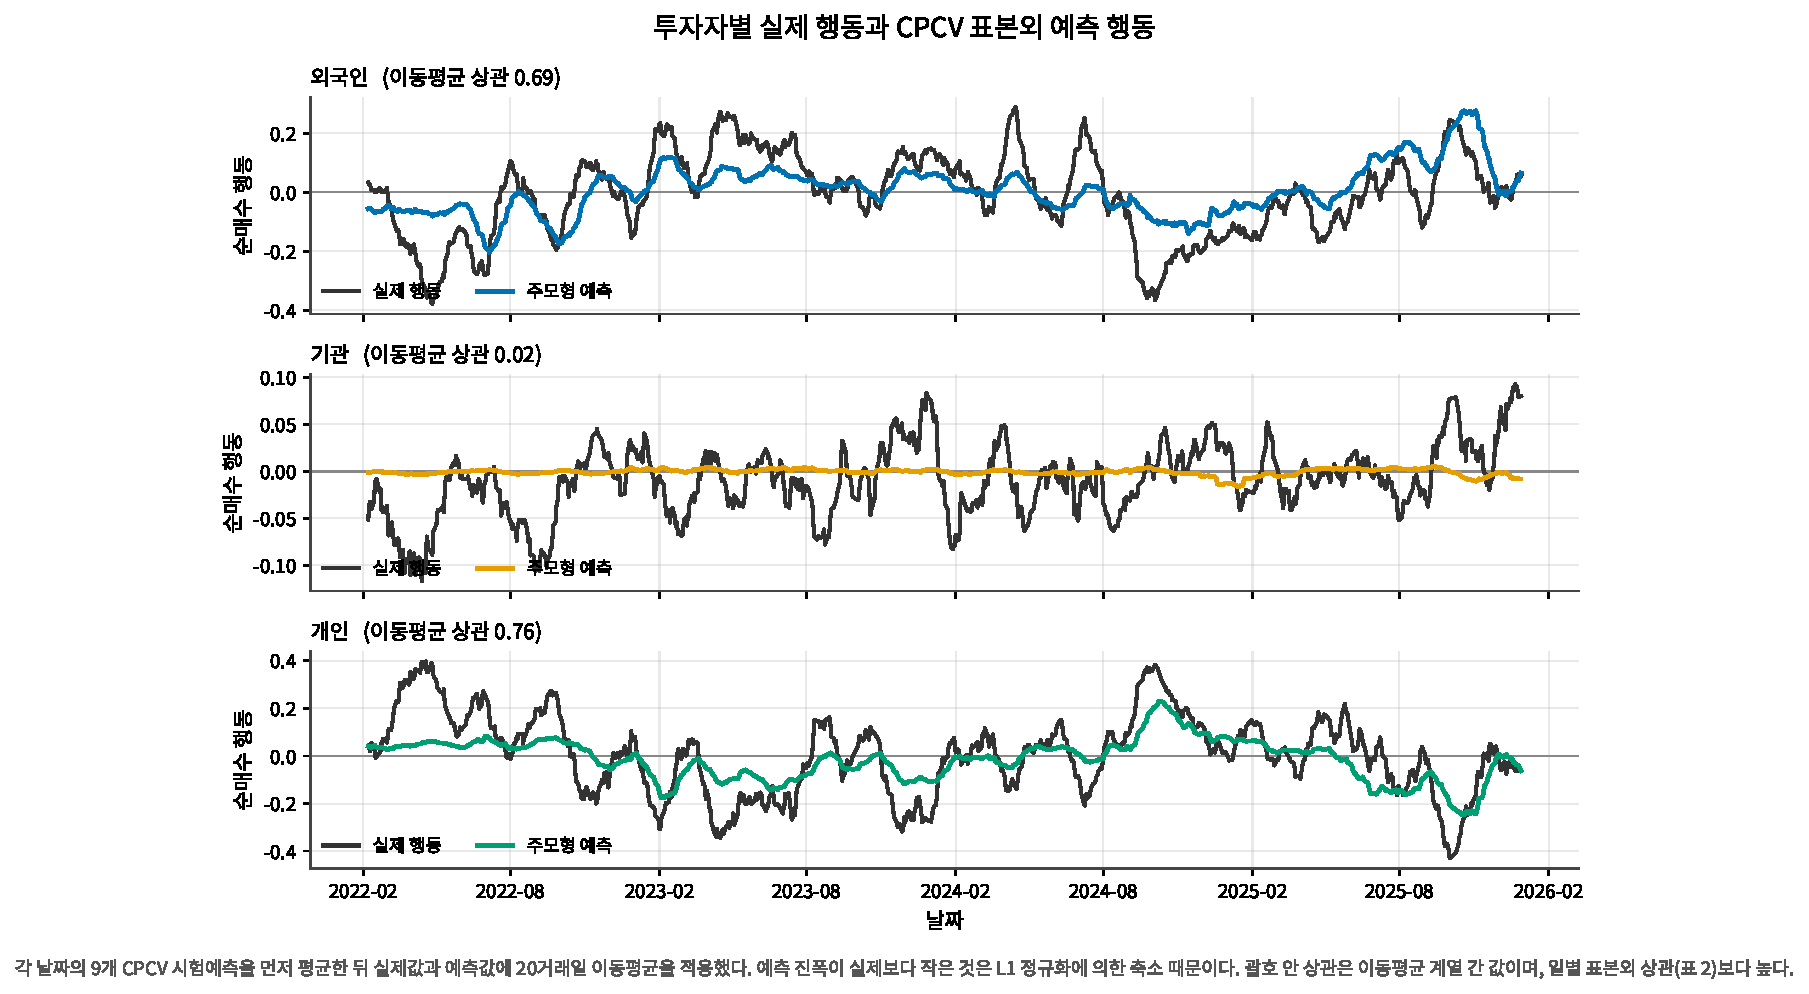
\includegraphics[width=\columnwidth]{figures/fig_actual_vs_prediction.pdf}
  \caption{Actual and out-of-sample predicted net buying (20-day moving average).
  The nine CPCV test predictions per date are averaged first. Correlations in the
  titles are between the smoothed series and are not directly comparable to the
  daily correlations in Table~\ref{tab:performance}.}
  \Description{Three line charts overlaying actual net buying and model
  predictions over time. In the institutional panel the prediction is flat near
  zero.}
  \label{fig:prediction}
\end{figure}

\begin{table}[t]
  \caption{Out-of-sample performance under CPCV (mean $\pm$ s.d.\ over 45
  splits) and the persistence baseline}
  \label{tab:performance}
  \small
  \centering
  \begin{tabular}{@{}lccc@{}}
    \toprule
    Metric & Foreign & Inst. & Retail \\
    \midrule
    \multicolumn{4}{@{}l}{\emph{SPR-IRL}}\\
    Directional accuracy & $0.636\pm0.039$ & $0.542\pm0.038$ & $0.608\pm0.044$ \\
    Correlation          & $0.278\pm0.110$ & $0.068\pm0.064$ & $0.245\pm0.118$ \\
    MAE                  & $0.195\pm0.019$ & $0.094\pm0.008$ & $0.264\pm0.029$ \\
    MAE / action s.d.    & $0.759$ & $0.756$ & $0.791$ \\
    Saturation rate      & $0.000$ & $0.000$ & $0.000$ \\
    \addlinespace
    \multicolumn{4}{@{}l}{\emph{Persistence} ($a_{t+1}\!\leftarrow\!a_t$)}\\
    Directional accuracy & $\mathbf{0.642}$ & $\mathbf{0.547}$ & $\mathbf{0.616}$ \\
    Correlation          & $\mathbf{0.359}$ & $\mathbf{0.136}$ & $\mathbf{0.311}$ \\
    \bottomrule
  \end{tabular}
\end{table}

In Figure~\ref{fig:prediction} the foreign and retail predictions track the
regime turns of the actual series (smoothed correlations 0.69 and 0.76) with a
smaller amplitude due to $L_1$ shrinkage, while the institutional prediction is
essentially pinned to zero (0.02).

Table~\ref{tab:performance} shows two things. First, dispersion across splits is
large, so types cannot be compared from a single split. Second, \textbf{the naive
persistence baseline beats SPR-IRL on directional accuracy and correlation}.
Since $a_t$ is published after the day-$t$ close this is an informationally
feasible rule. The reason is clear: the action has autocorrelation
$0.401/0.149/0.345$, yet the feature set contains no lagged own action.
Restricting the features to (F1)--(F3) was a design choice ensuring that all
types share only features corresponding to independently established
regularities, not a design for predictive performance.
Table~\ref{tab:performance} shows that the model has not merely fitted noise; it
is not evidence of predictive superiority.

Because the saturation rate is zero for every type and split, the premise of
Proposition~\ref{prop:lasso} holds and the estimator is literally a Lasso.

\subsection{Recovered Preferences: A Mirror Image}
\label{sec:beta}

\begin{figure*}[t]
  \centering
  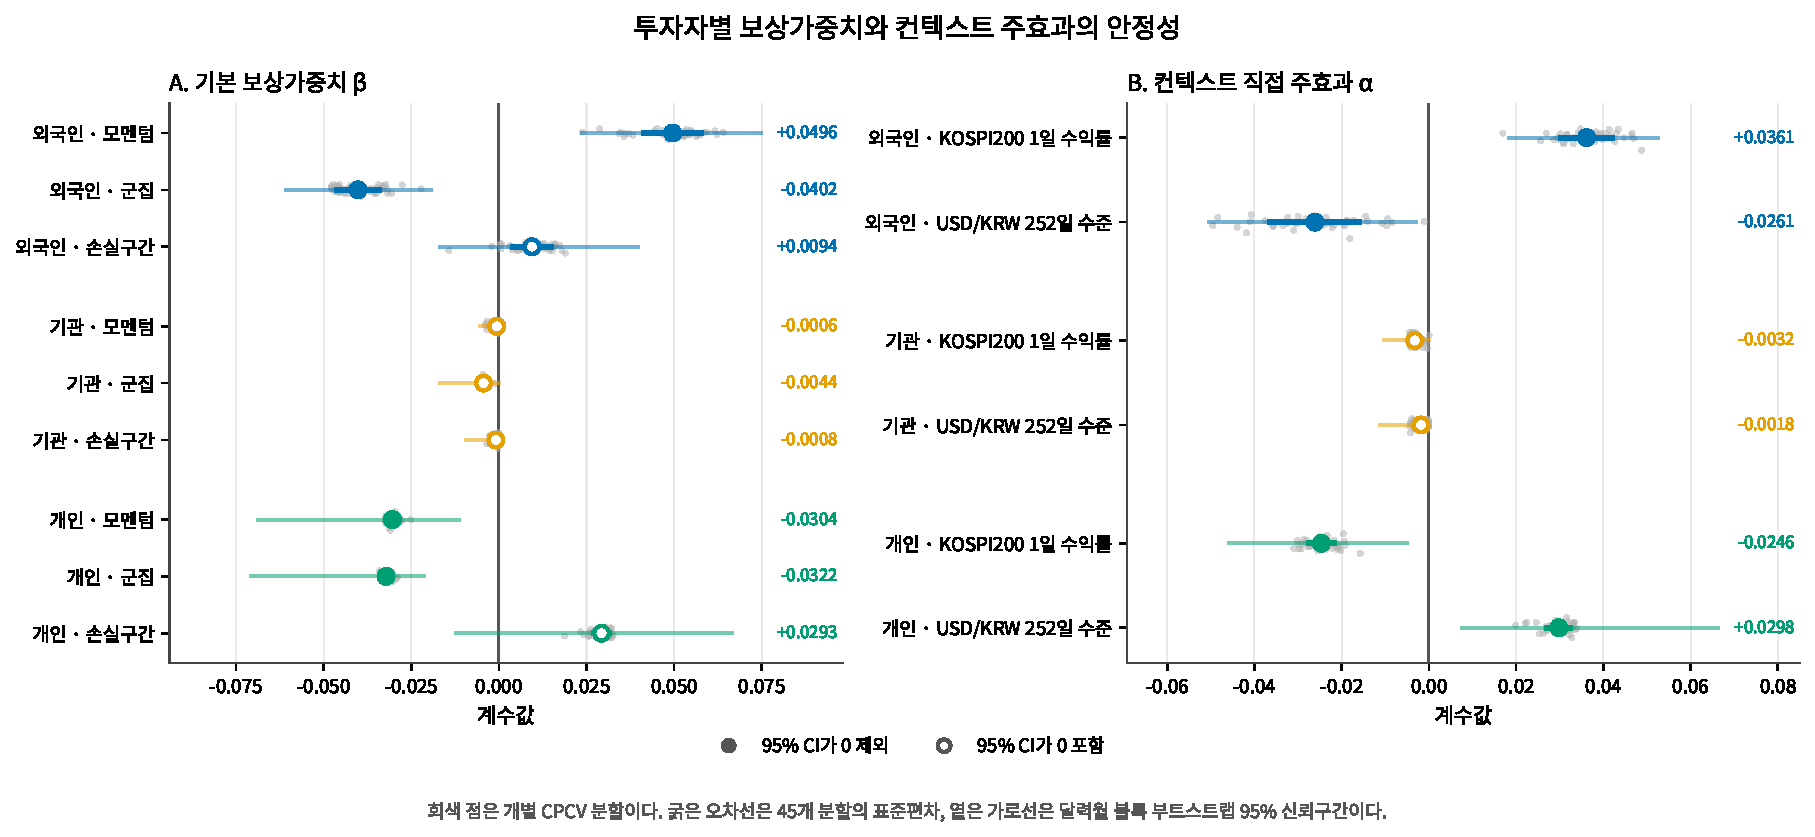
\includegraphics[width=\textwidth]{figures/fig_beta_alpha_forest.pdf}
  \caption{Stability of the recovered baseline reward weights $\beta$ (A) and
  context main effects $\alpha$ (B). Grey dots are the 45 individual CPCV splits,
  thick error bars the across-split standard deviation, and light horizontal
  lines the 95\% calendar-month block bootstrap interval. Hollow markers denote
  terms whose interval contains zero.}
  \Description{Two forest-plot panels. Panel A gives momentum, herding and
  underwater coefficients for the three types; panel B gives the KOSPI200 and FX
  main effects. Foreign momentum is positive, retail momentum negative, and every
  institutional marker is hollow.}
  \label{fig:forest}
\end{figure*}

\textbf{The mirror image on momentum.} The foreign momentum weight is $+0.0496$
and positive in all 45 splits; the retail weight is $-0.0304$ and negative in all
45. Their bootstrap intervals do not overlap and each excludes zero
(Figure~\ref{fig:forest}A). Although the same feature set was estimated
independently for each type, the two diverge in opposite directions, matching the
sign expectations of prior
work~\cite{grinblatt2000investment,choe1999foreign}.

\textbf{Reappearance in the context response.} The same mirror appears in the
main effects (Figure~\ref{fig:forest}B). Foreign investors move toward net buying
when the market rises ($+0.0361$) and toward net selling when the won is weak
($-0.0261$); retail investors do the opposite on both ($-0.0246$, $+0.0298$). All
four keep their sign in all 45 splits and all four intervals exclude zero.

\textbf{Herding.} The herding coefficient is negative in all 45 splits for all
three types, and the foreign ($-0.0402$) and retail ($-0.0322$) intervals exclude
zero. This does not separate a behavioural interpretation from the
market-clearing constraint: under the $-0.77$ same-day correlation of
\S\ref{sec:data}, much of the negative coefficient may be mechanical. We
therefore restrict the result to the descriptive statement that observed
aggregate flow shows a negative cross-type association, and the same reservation
applies to the mirrored main effects.

\textbf{Underwater.} The retail underwater weight is $+0.0293$ and positive in
all 45 splits, consistent with the reference-price dependence of the
disposition-effect
literature~\cite{shefrin1985disposition,odean1998investors}. However, as
Figure~\ref{fig:forest}A shows, the interval contains zero for all three types.
The retail interval is $[-0.0122,+0.0665]$: although the sign is 100\% consistent
across splits, it flips in 5.5\% of month-block resamples. This is precisely the
situation anticipated in \S\ref{sec:protocol}, where sign consistency understates
uncertainty because splits share observations. We therefore report a sign
consistent with the disposition effect without claiming it as established.

Of the twelve interaction coefficients, four keep their sign in all 45 splits
(foreign momentum $\times$ KOSPI200 $-0.0139$; retail momentum $\times$ FX
$+0.0144$; retail herding $\times$ KOSPI200 $-0.0080$; retail underwater $\times$
FX $-0.0186$), of which the first and last also pass the bootstrap. Since twelve
were examined jointly, we present them as exploratory only.

\subsection{Stability}
\label{sec:stability}

\begin{figure*}[t]
  \centering
  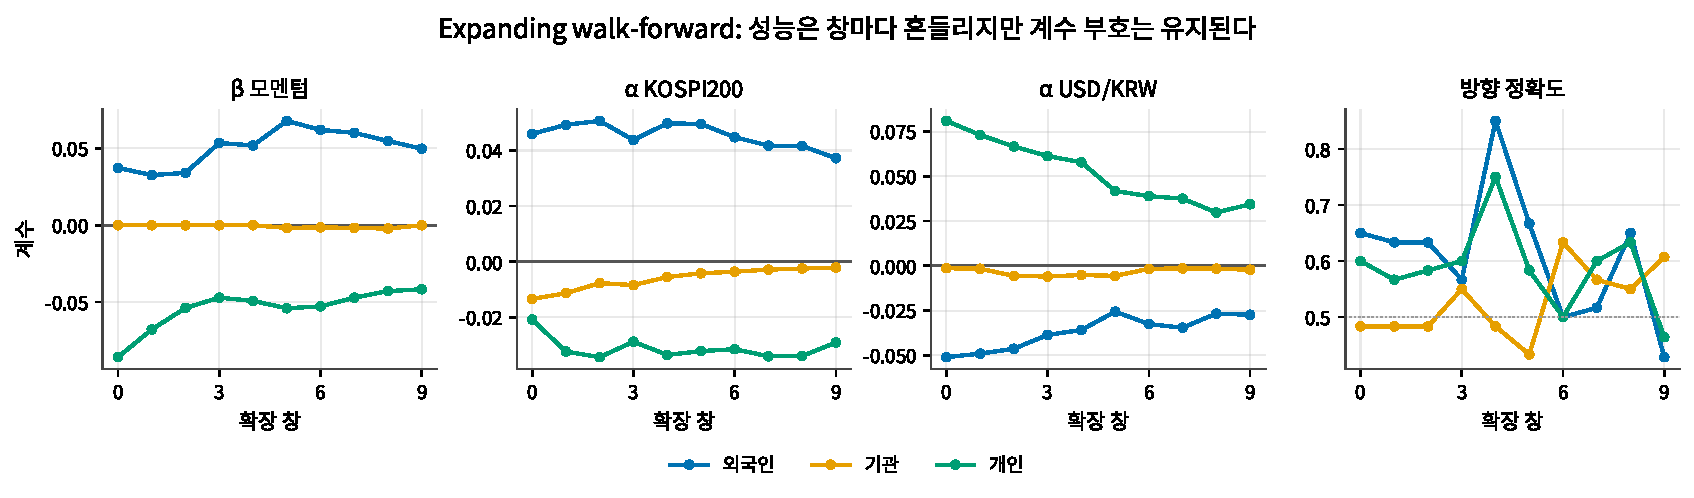
\includegraphics[width=\textwidth]{figures/fig_walk_forward.pdf}
  \caption{Coefficient paths and directional accuracy over ten expanding
  walk-forward windows. Performance fluctuates while the signs hold, and the
  foreign and retail momentum paths never cross.}
  \Description{Four line charts against the expanding-window index showing the
  momentum coefficient, two context main effects, and directional accuracy for
  the three types.}
  \label{fig:walkforward}
\end{figure*}

\textbf{(V2)} The bootstrap splits the results three ways: the eight terms
forming the momentum and context mirrors all exclude zero, the underwater weights
do not, and no institutional term does (the hollow markers in
Figure~\ref{fig:forest}).

\textbf{(V3)} In Figure~\ref{fig:walkforward} performance fluctuates sharply:
foreign directional accuracy moves between 0.43 and 0.85, averaging
$0.610\pm0.116$, and the correlation falls to $0.131\pm0.162$, less than half the
CPCV value of 0.278. Because CPCV can place a test fold ahead of a training fold
while walk-forward cannot, we report this degradation as a generalization limit
from the temporal structure. The coefficient paths, by contrast, do not
fluctuate: foreign momentum is positive in all ten windows and retail negative in
all ten, the two never cross, and the same mirror holds for both context main
effects. The institutional paths hug the zero line.

\textbf{(V4)} Foreign and retail coefficients agree to four decimal places under
$L_1$, $L_2$ and no penalty, so the mirror is not an artefact of the penalty.
Only the institutional coefficients move (herding
$-0.0076\rightarrow-0.0124$, underwater $-0.0000\rightarrow-0.0018$).

\subsection{Institutional Investors: A Converged Null}
\label{sec:null}

For institutional flow SPR-IRL finds no preference that is stably identified at
daily frequency, and we report this as a result. The evidence is fivefold:
(i) the prediction series degenerates to zero (Figure~\ref{fig:prediction});
(ii) excluding herding, the coefficients are about one fortieth of the other
types ($-0.0006$, $-0.0008$); (iii) no term excludes zero in the bootstrap
(Figure~\ref{fig:forest}); (iv) the coefficients depend on the choice of penalty;
and (v) momentum sign consistency is 40\% of ten walk-forward windows and
underwater 0\%.

\textbf{This null is not an optimization failure.} By
Proposition~\ref{prop:lasso}, Equation~\eqref{eq:loss} is convex with a unique
global optimum, and comparing the solution reached against the closed-form
optimum of the same objective leaves an institutional gap of only 0.17\% on
average and 0.48\% at most (0.21\% for foreign, 0.92\% for retail). All three
types reach the attainable optimum; only for institutional investors do the
coefficients there sit near zero. The data do not determine an institutional
preference; the optimizer did not fail to find one.

Economically this reads naturally: the ``institutional'' category aggregates
pension funds, investment trusts, insurers, private funds and securities firms,
so flows from agents with different objectives offset one another.

\subsection{Construct Validity}
\label{sec:construct}

\begin{table}[t]
  \caption{Prior sign expectations and recovered results}
  \label{tab:construct}
  \small
  \begin{tabular}{@{}>{\raggedright\arraybackslash}p{0.28\columnwidth}
                  >{\raggedright\arraybackslash}p{0.13\columnwidth}
                  >{\raggedright\arraybackslash}p{0.28\columnwidth}
                  >{\raggedright\arraybackslash}p{0.15\columnwidth}@{}}
    \toprule
    Regularity & Expected & Recovered & Verdict \\
    \midrule
    Foreign trend trading~\cite{grinblatt2000investment,choe1999foreign}
      & $\beta^{mom}\!>\!0$ & $+0.0496$ (100\%, CI excl.\ 0) & matches \\
    Retail contrarian~\cite{grinblatt2000investment,kaniel2008individual}
      & $\beta^{mom}\!<\!0$ & $-0.0304$ (100\%, CI excl.\ 0) & matches \\
    Disposition effect~\cite{shefrin1985disposition,odean1998investors}
      & $\beta^{uw}\!>\!0$ & $+0.0293$ (100\%, CI incl.\ 0) & partial \\
    Institutional herding~\cite{lakonishok1992impact}
      & $\beta^{herd}\!>\!0$ & $-0.0044$ (100\%, CI incl.\ 0) & mismatch \\
    \bottomrule
  \end{tabular}
\end{table}

Table~\ref{tab:construct} reports the contrast. That the recovered signs agree
with independently established regularities, and that two types diverge in
opposite directions on momentum, is evidence of construct validity given that
all types shared the same features and model form. The mismatch arises because
the measured object differs: Lakonishok et al.~\cite{lakonishok1992impact}
measure herding \emph{within} the institutional group, whereas
Equation~\eqref{eq:herd} measures whether institutions move with the
\emph{other two types}, so our result is not a refutation of that literature.
